%!TeX TS-program = pdflatex
%!TeX encoding = UTF-8 Unicode
%!TeX spellcheck = en-US
%!BIB TS-program = bibtex
% -*- coding: UTF-8; -*-
% vim: set fenc=utf-8
%: METADATA
%: %%%%%%%%%%%%%%%%%%%%%%%%%%%%%%%%%%%%%%%%%%%%%%%%%%%%%%%%%%%%%%%%%%%%
\newcommand{\AuthorA}{Chlo\'e Pasturel}
\newcommand{\AuthorB}{Anna Montagnini}%
\newcommand{\AuthorC}{Laurent U.~Perrinet}%
\newcommand{\Address}{Institut de Neurosciences de la Timone, CNRS / Aix-Marseille Universit\'e - Marseille, France}%
\newcommand{\Website}{http://invibe.net/LaurentPerrinet}%
\newcommand{\Email}{Laurent.Perrinet@univ-amu.fr}%
\newcommand{\Title}{
%Principles and psychophysics of Active Inference in anticipating a dynamic probabilistic bias
Humans adapt to the volatility of visual motion properties, and know about it
%Anticipating a volatile probabilistic bias in visual motion direction
%Humans adapt to the volatility of visual motion properties :  eye movements and explicit guesses
}
\newcommand{\Acknowledgments}{PACE-ITN - code and material @ \url{\Website/Publications/Pasturel_etal2018}. TODO: RIck + Karl + JB + Laurent Madelain }
\newcommand{\Abstract}{
The brain has to constantly adapt to changes in the environment,
for instance when a contextual probabilistic variable switched its state.
For an agent interacting with such an environment,
it is important to respond to such switches with the shortest delay.
However, this operation has in general to be done with noisy sensory inputs
and solely based on the information available at the present time.
Here, we tested the ability of humans observers to accurately anticipate,
with their eye movements,
a target's motion direction
throughout random sequences of rightward/leftward motion alternations,
with random-length contextual blocks of different biases in direction probability.
Experimental results were compared to
those of a probabilistic agent optimized
with respect to this switching model.
We found a better fit between
the behaviorally observed anticipatory response
with that of the probabilistic agent
compared to other models such as the leaky-integrator model.
Moreover, we could similarly fit
the level of confidence given by human observers
with that provided by the model and
draw a common marker for subject inter-variability,
titrating their level of preference between exploration and exploitation.
Such results provide evidence that
human observers may efficiently represent an anticipatory belief
along with its precision and
they support a novel approach to more generically test
human cognitive abilities in uncertain and dynamic environments.
}
%%%%%%%%%%%%%%%%%%%%%%%%%%%%%%%%%%%%%%%%%%
\documentclass[profile,final,english, draft]{article}%
\usepackage{babel}
% MATHS (AMS)
\usepackage{amsmath}
\usepackage{amsfonts}
\usepackage{amssymb}
\usepackage{amsthm}
\newcommand{\KL}[2]{\text{KL}( #1 | #2 )}
%% parenthesis
\newcommand{\pa}[1]{\left( #1 \right)}
\newcommand{\bpa}[1]{\big( #1 \big)}
\newcommand{\choice}[1]{ %
	\left\{ %
		\begin{array}{l} #1 \end{array} %
	\right. }
% ensembles
\newcommand{\ens}[1]{ \{ #1 \} }
\newcommand{\enscond}[2]{ \left\{ #1 \;;\; #2 \right\} }
% egal par définition
\newcommand{\eqdef}{\ensuremath{\stackrel{\mbox{\upshape\tiny def.}}{=}}}
\newcommand{\eqset}{\ensuremath{\stackrel{\mbox{\upshape\tiny set}}{=}}}
\newcommand{\eq}[1]{\begin{equation*}#1\end{equation*}}
\newcommand{\eql}[1]{\begin{equation}#1\end{equation}}

\DeclareMathOperator{\argmin}{argmin}
\DeclareMathOperator{\argmax}{argmax}
\newcommand{\uargmin}[1]{\underset{#1}{\argmin}\;}
\newcommand{\uargmax}[1]{\underset{#1}{\argmax}\;}
\newcommand{\umin}[1]{\underset{#1}{\min}\;}
\newcommand{\umax}[1]{\underset{#1}{\max}\;}
\newcommand{\usup}[1]{\underset{#1}{\sup}\;}
% for units
\usepackage{siunitx}%
\newcommand{\ms}{\si{\milli\second}}%

%% Symboles arrondis
\newcommand{\Aa}{\mathcal{A}}
\newcommand{\Bb}{\mathcal{B}}
\newcommand{\Cc}{\mathcal{C}}
\newcommand{\Dd}{\mathcal{D}}
\newcommand{\Ee}{\mathcal{E}}
\newcommand{\Ff}{\mathcal{F}}
\newcommand{\Gg}{\mathcal{G}}
\newcommand{\Hh}{\mathcal{H}}
\newcommand{\Ii}{\mathcal{I}}
\newcommand{\Jj}{\mathcal{J}}
\newcommand{\Kk}{\mathcal{K}}
\newcommand{\Ll}{\mathcal{L}}
\newcommand{\Mm}{\mathcal{M}}
\newcommand{\Nn}{\mathcal{N}}
\newcommand{\Oo}{\mathcal{O}}
\newcommand{\Pp}{\mathcal{P}}
\newcommand{\Qq}{\mathcal{Q}}
\newcommand{\Rr}{\mathcal{R}}
\newcommand{\Ss}{\mathcal{S}}
\newcommand{\Tt}{\mathcal{T}}
\newcommand{\Uu}{\mathcal{U}}
\newcommand{\Vv}{\mathcal{V}}
\newcommand{\Ww}{\mathcal{W}}
\newcommand{\Xx}{\mathcal{X}}
\newcommand{\Yy}{\mathcal{Y}}
\newcommand{\Zz}{\mathcal{Z}}
%% ========  polices de caracteres =============
\usepackage[T1]{fontenc}%
\usepackage{lmodern}%
\usepackage{t1enc}
\usepackage{ragged2e}
%============ graphics ===================
\usepackage[pdftex]{graphicx}%
\DeclareGraphicsExtensions{.pdf,.png,.jpg}%
\graphicspath{{../figures/}, {./figures/}}% TODO remove {./figures/},  at the end
%============ bibliography ===================

\usepackage{filecontents}
% --------------------------------------------------------------------------
% --------------------------------------------------------------------------
% --------------------------------------------------------------------------
\begin{filecontents}{Pasturel_etal2018.bib}

@article{Meyniel13,
abstract = {
No pain, no gain: cost-benefit trade-off has been formalized in classical decision theory to account for how we choose whether to engage effort. However, how the brain decides when to have breaks in the course of effort production remains poorly understood. We propose that decisions to cease and resume work are triggered by a cost evidence accumulation signal reaching upper and lower bounds, respectively. We developed a task in which participants are free to exert a physical effort knowing that their payoff would be proportional to their effort duration. Functional {\{}MRI{\}} and magnetoencephalography recordings conjointly revealed that the theoretical cost evidence accumulation signal was expressed in proprioceptive regions (bilateral posterior insula). Furthermore, the slopes and bounds of the accumulation process were adapted to the difficulty of the task and the money at stake. Cost evidence accumulation might therefore provide a dynamical mechanistic account of how the human brain maximizes benefits while preventing exhaustion.
},
author = {Meyniel, Florent and Sergent, Claire and Rigoux, Lionel and Daunizeau, Jean and Pessiglione, Mathias},
doi = {10.1073/pnas.1211925110},
issn = {1091-6490},
journal = {Proceedings of the National Academy of Sciences of the United States of America},
keywords = {decision-making},
number = {7},
pages = {2641--2646},
pmid = {23341598},
title = {{Neurocomputational account of how the human brain decides when to have a break.}},
url = {http://dx.doi.org/10.1073/pnas.1211925110},
volume = {110},
year = {2013}
}

%Montagnini A, Souto D, and Masson GS (2010) <a href="http://jov.arvojournals.org/article.aspx?articleid=2138664">J Vis (VSS Abstracts) 10(7):554</a>,<BR> Montagnini A, Perrinet L, and Masson GS (2015) <a href="https://arxiv.org/abs/1611.07831">BICV book chapter</a>

@article{Montagnini2010,
author = {Montagnini, Anna and Souto, David and Masson, Guillaume S},
journal = {Journal of Vision},
keywords = {bicv-motion},
number = {7},
pages = {554},
title = {{Anticipatory eye-movements under uncertainty: a window onto the internal representation of a visuomotor prior}},
volume = {10},
year = {2010}
}

@article{AdamsMackay2007,
author = {{Prescott Adams}, R. and {MacKay}, D.~J.~C.},
title = "{Bayesian Online Changepoint Detection}",
journal = {ArXiv e-prints},
archivePrefix = "arXiv",
eprint = {0710.3742},
primaryClass = "stat.ML",
keywords = {Statistics - Machine Learning},
year = 2007,
month = oct,
adsurl = {http://adsabs.harvard.edu/abs/2007arXiv0710.3742P},
adsnote = {Provided by the SAO/NASA Astrophysics Data System}
}
}
\end{filecontents}
%\usepackage[numbers,comma,sort&compress,round]{natbib} %
\usepackage[%style=nature,
maxcitenames=2,
maxnames = 2,
firstinits=true,
uniquename=init,
sorting=none,
url=false,
isbn=false,
eprint=false,
texencoding=latin1,
bibencoding=utf8,
autocite=superscript,
backend=bibtex,
%articletitle=false
]{biblatex}%
\addbibresource{Pasturel_etal2018.bib}%
\newcommand{\citep}[1]{\parencite{#1}}
\newcommand{\citet}[1]{\textcite{#1}}
%%%%%%%%%%%%%%%%%%%%%%%%%%%%%%
%% OPTIONAL MACRO FILES
\usepackage{tikz}
%\usepackage{tikz,tkz-euclide} \usetkzobj{all} % loading all objects
%\usetikzlibrary{positioning} \usetikzlibrary{calc}
%\usepackage{sfmath}
\newcommand{\seeFig}[1]{see Figure~\ref{fig:#1}}
\newcommand{\seeEq}[1]{see Equation~\ref{eq:#1}}
\newcommand{\seeApp}[1]{see Appendix~\ref{app:#1}}
\newcommand{\seeSec}[1]{see Section~\ref{sec:#1}}
%============ hyperref ===================
\usepackage[unicode,linkcolor=red,citecolor=red,filecolor=black,urlcolor=red,pdfborder={0 0 0}]{hyperref}%
\hypersetup{%
pdftitle={\Title},%
pdfauthor={\AuthorA},%< \Email > \Address},%
}%
\usepackage{color}%
%%%%%%%%%%%%%%%%%%%%%%%%%%%%%%%%%%%
\title{\Title}%
\author{\AuthorA,
\AuthorB,
\AuthorC\thanks{\Address} }

%%%%%%%%%%%% Her begynner selve dokumentet %%%%%%%%%%%%%%%
\begin{document}%
\maketitle%
%%%%%%%%%%%%%%%%%%%%%%%%%%%%%%%%%%%%%%%%%%%%%%%%%%%%%%%%%%%%%%%%
%: Abstract
\begin{abstract}
\Abstract
\end{abstract}
%: %%%%%%%%%%%%%%%%%%%%%%%%%%%%%%%%%%%%%%%%%%%%%%%%%%%%%%%%%%%%%%%
\section{Motivation}
%%%%%%%%%%%%%%%%%%%%%%%%%%%%%%%%%%%%%%%%%%%%%%%%%%%%%%%%%%%%%%%%
%%%%%%%%%%%%%%%%%%%%%%%%%%%%%%%%%%%%%%%%%%%%%%%%%%%%%%%%%%%%%%%%
%%%%%%%%%%%%%%%%%%%%%%%%%%%%%%%%%%%%%%%%%%%%%%%%%%%%%%%%%%%%%%%%
\subsection{Volatility of sensory contingencies and
the adaptation of cognitive systems}
% --------------------------------------------------------------------------------------
% /!\ some parts of this subsection remotely originate from JB's thesis...
%: general volatility and perceptual learning
We live in a fundamentally volatile world for which
our cognitive system has to constantly adapt.
Think for instance of the variability of environmental contingencies
present in global climate and
the probability of a change in its dynamic
since the switch of civilization in an industrialized organization:
We have access to (possibly noisy and heterogeneous) measurements
of some (few) markers, such as carbon dioxide concentration and
wish to predict the range of the mean temperature on Earth.
This reveals some of the dynamics of
the complex system constituted by the atmosphere
and of acceptable levels of temperature for civilization.
Based on past history and prior knowledge about
the effect of our own emissions of carbon dioxide
(for instance priming evidence of the link between carbon dioxide
concentration and an elevation of temperature),
one should be able to predict at best if either
one could continue to exploit a similar strategy (emit gases)
or if it is necessary to explore different paradigms (limit emissions).
% * the evolution  of prices on the stock market: Any Socio-economic contextual index may make the price evolve up or down, slowly or more Rapidly
% * ecological change
% * the side (left or right of the field) in which the ball is on a soccer field
Such a strategy is effective at this large scale level
but also at all levels which are behaviorally relevant,
such as contextual changes in our everyday life.
Infer near future state in a dynamic environment ---
or at least to form beliefs as precise as possible
about a future environmental context ---
are ubiquitous to cognitive systems
such that one can act upon them at the present time~\citep{ref}..
In the long term, such capacity is essential to the adaptation
of the behavior through reinforcement learning~\citep{ref}.
In visual psychophysics, that is,
in controlled experimental settings challenging visual perception,
such adaptive processes have been mostly put in evidence
by analyzing the history in a sequence of experimental trials,
such that one could put them in evidence
at the time scale of one to several minutes.

%: Past history of sensory event integration in vision
Indeed, stimulus history of visual events influences
how current stimuli are perceived and acted upon.
One putative purpose is to reduce
the sensitivity to recurrently presented stimuli and
thus to re-calibrate perceptual experience~\citep{Clifford2007, Webster2011, Kohn2007}.
Recent examples of positive biases in perceptual discrimination are
numerous and show that the visual system tends
to favor stimulus' temporal and spatial stability:
For instance, facilitatory effects such as priming
enhance the stimulus identification of repeated motion~\citep{Verstraten1994, Tiest2009}.
% An example, is Priming: Repeated stimulations
% creates a facilitation in perception~\citep{Kristjnsson2010WherePM, Maljkovic1994, Tulving1990}.
% Indeed, after exposure to a similar stimulus,
% priming leads to faster responses in perceptual detection or identification of probes.
% It also occurs specifically for visual motion stimuli~\citep{Anstis1987, Campana2002, Pinkus1997}.
This type of perceptual learning mainly produces improvements in discrimination
with long-term training on a perceptual judgement~\citep{Lu2009}.
The ability to detect sequential regularities
thus appears as a fundamental ability
for the adaptive behavior of species.
A same response presented several times could indeed
lead to faster and more accurate responses and,
on the other hand, lead to impairment in the behavior
when a presented stimulus was going
against the expected belief~\citep{Hyman1953, Yu2009}.
This process is highly dynamic especially in complex environments
where new contingencies can arise at every moment.
% In the case of visual motions,
% the process of visual adaptation in mostly defined
% by repeated exposures of stimuli and
% after-effects related to those statistical regularities~\citep{Thompson2009}.
% An example, is Motion Aftereffect:
% Prolonged exposure to a stimulus moving in one direction results
% in a motion aftereffect: a stationary stimulus is perceived to move
% in the opposite direction as the adapting stimulus~\citep{Anstis1998, Mather2011}.
% The motion aftereffect usually builds up over time~\citep{Hershenson1993},
% sometimes after relatively short exposures~\citep{Kanai2005, Pavan2010}
% and can last for period of ten seconds~\citep{Anstis1998}.
One remaining question though, is to understand why
this adaptation occur in cognitive systems and
in particular why they may deviate
in some pathological disorders such as schizophrenia~\citep{Adams2010}.
There is therefore a necessity to select
a modeling approach to best understand the function of such phenomena
and in particular how such sequential effects are integrated.
At present, Bayesian inference is an effective methodology
to deal with this question.

%: Bayesian methods & role of predictive processing for this adaptive response
In all generality, Bayesian methods allow to propose and quantitatively assess
a range of hypothesis about the processing
of available information by observers~\citep{Deneve1999, Diaconescu2014, Deaunizau}.
A key principle in the Bayesian inference approach is
that each stated hypothesis is quantitatively formalized
such that measurements and outcomes may be linked by
a generic probabilistic model. %, the generative model.
This model is parameterized by some structural variables
(such as weights, non-linear gain functions or prior knowledge)
and some relevant latent variables
which may be represented as probabilities.
Then, using the rules of probability calculus
one can progressively update beliefs about the latent variables,
such that one can finally infer the hidden structure of received inputs~\citep{Hoyer2003, Ma2014}.
For instance, using Bayes's rule one can combine
the likelihood of observations given the generative model and
the prior of these latent variables~\citep{Janes2014}.
Of particular interest for us is the possibility to
quantitatively represent
the predictive and iterative nature of the probabilistic model.
Indeed, once the belief about latent variables
is formed from the sensory input,
this belief can be used to update
the prior over of future beliefs on latent variables~\citep{Montagnini2007}
Thus, the comparisons between expectations and actual data produces
a constant update the estimates of the model under a mechanism
that is labelled as the~\textit{active inference}~\citep{Friston2003, Friston2010}.
Such methodology thus allows to infer present latent variables
but also to understand longer time effects such as adaptation and learning
through variational inference over
the parameters of the probabilistic model~\citep{ref}.
In a recent study,~\citet{Meyniel2016} simulated
a model over five different set of datas
previously published~\citep{Squires1976, Huettel2002, Kolossa2013, Cho2002, Falk1997}.
Their main conclusion was that
a learning of local transition probabilities
was sufficient to explain the large repertoire
of experimental effects reported in these studies.
They concluded that transitions probabilities constitute
a core building block of sequence knowledge in the brain,
which then applies to a variety of sensory modalities and
experimental situations.
As such sequential effects in binary sequences are better explained
by a learning of transition probabilities
than of the absolute item frequencies or the frequencies of their alternations.
The critical difference lies in the content
of what is learned (item frequencies versus transition probabilities).
More generally, Bayesian models may consider
a vast hypothesis space~\citep{Kemp2008} and
then attempt to capture human behavior.
%Chopin and %Mamassian and the use of visual confidence  (see Ann rev of Vision 2016)
Interestingly, the observation of priming effects
have been observed for anticipatory smooth eye movements (aSPEM)
and therefore allow for the such predictive processes. %
% --------------------------------------------------------------------------------------
\subsection{Anticipatory SPEM (aSPEM)}
% --------------------------------------------------------------------------------------
%-------------------------------------------------------------%
%: FIGURE 1 fig:intro
\begin{figure}%[b!]
\centering{
\begin{tikzpicture}%[thick,scale=1, every node/.style={scale=1} ]
% cf 0_protocole.ipynb
\node [anchor=north west]  (img2) at (0.000\linewidth,.618\linewidth){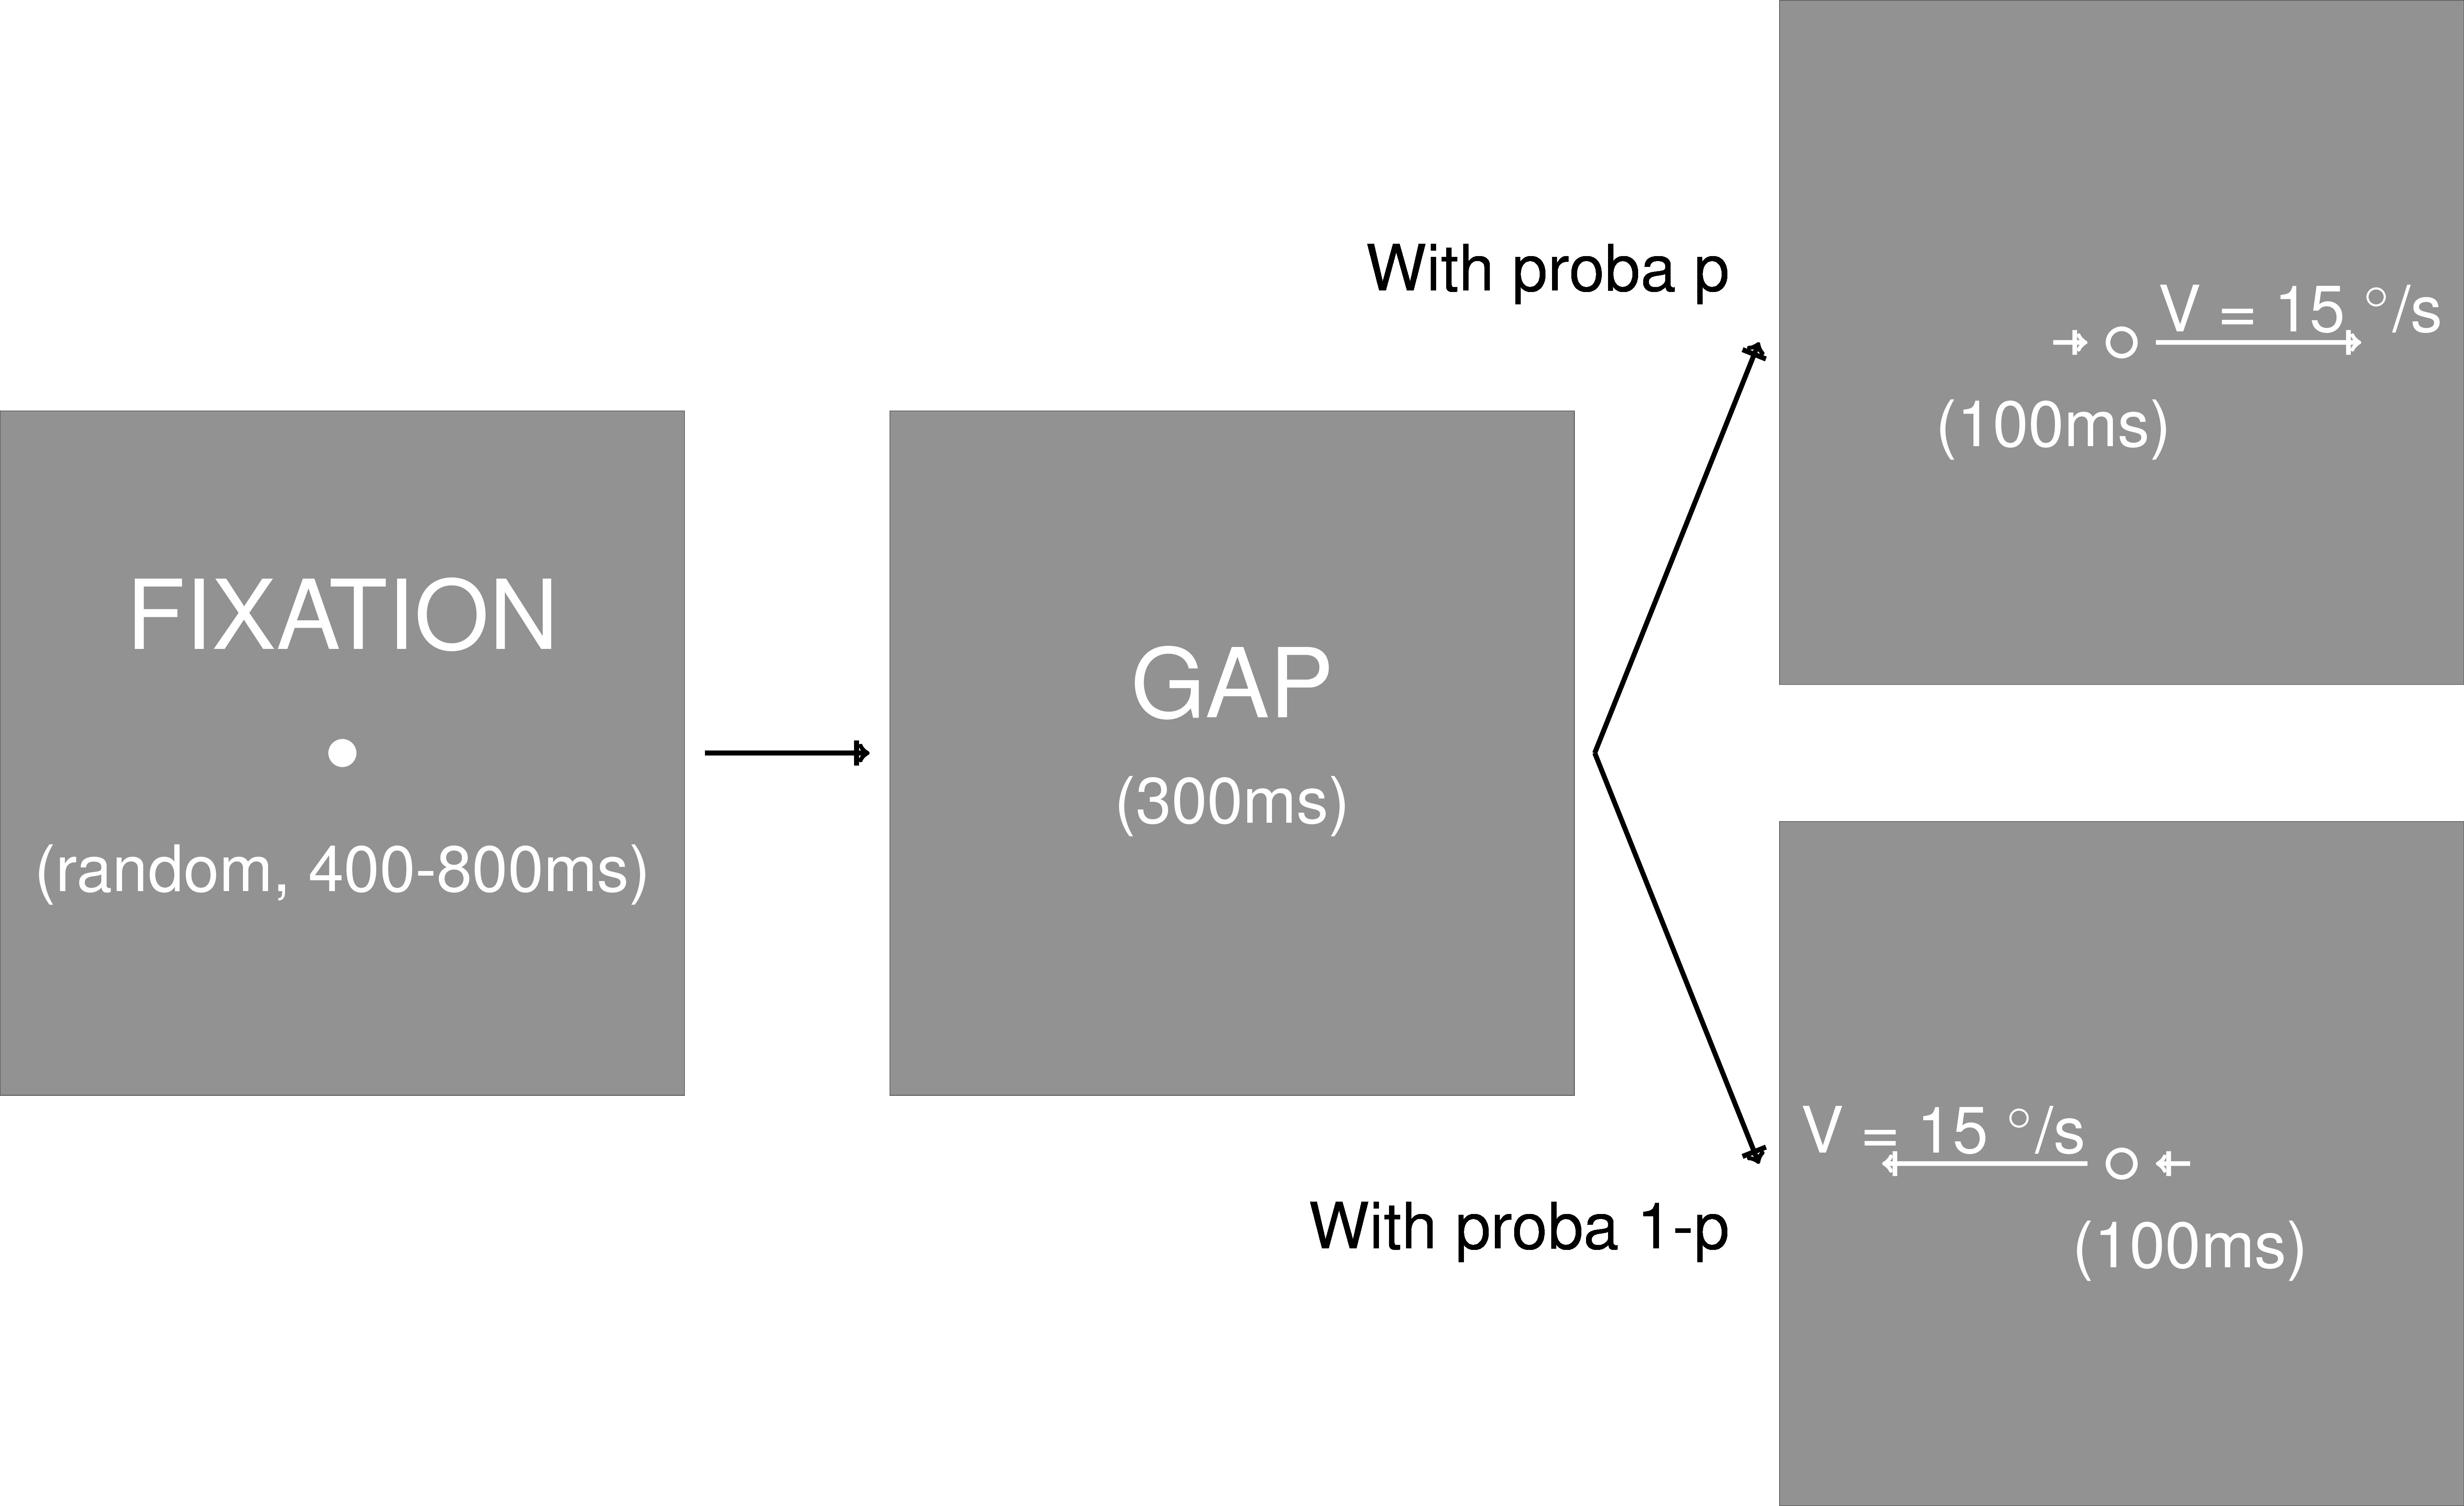
\includegraphics[width=0.333\linewidth]{protocol_recording}};
% cf 3_Results_2.ipynb ??
\node [anchor=north west]  (img2) at (0.333\linewidth,.618\linewidth){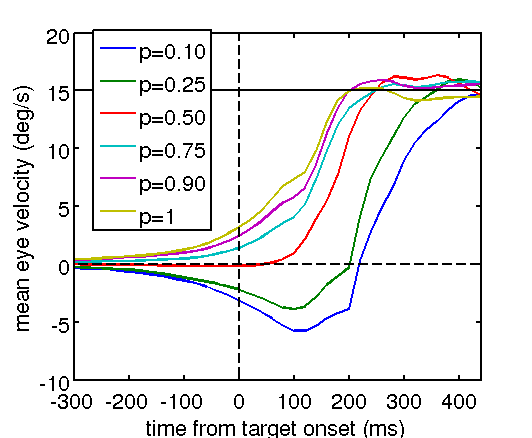
\includegraphics[width=0.333\linewidth]{image_anna_1}};
% cf 0_protocole.ipynb
\node [anchor=north west]  (img2) at (0.666\linewidth,.618\linewidth){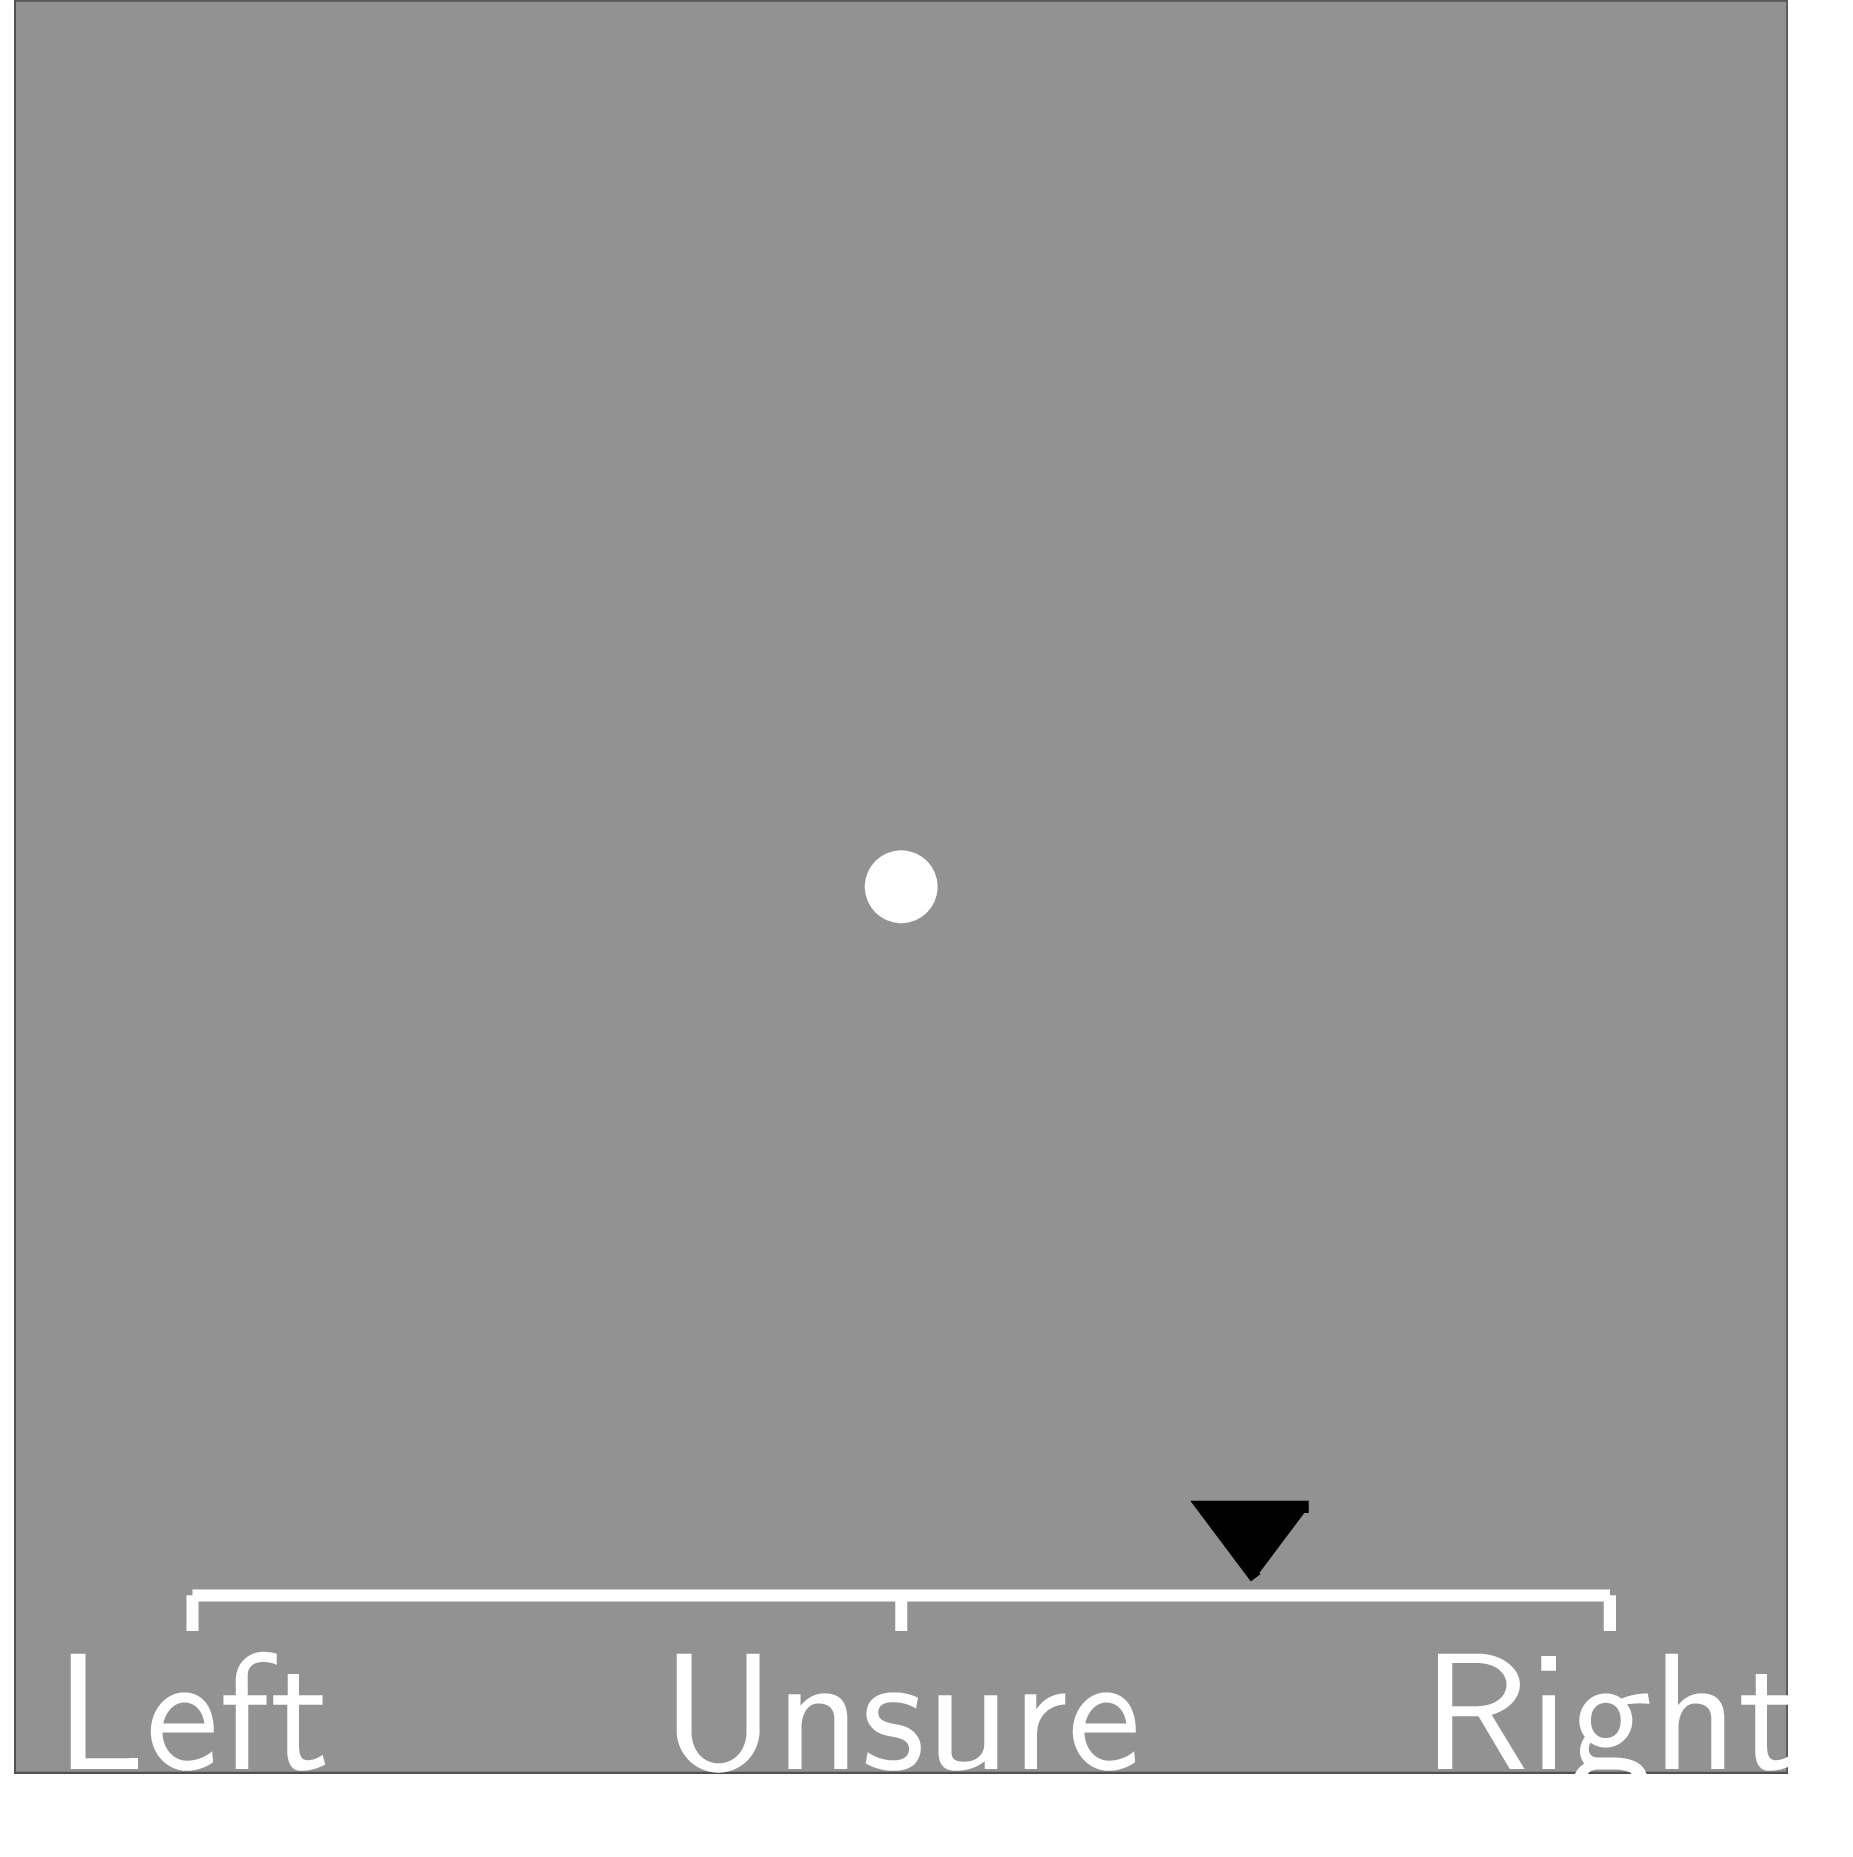
\includegraphics[width=0.25\linewidth]{protocol_bet_simple}};
\draw [anchor=north west] (0.000\linewidth, .618\linewidth) node {$\mathsf{(A)}$};
\draw [anchor=north west] (0.333\linewidth, .618\linewidth) node {$\mathsf{(B)}$};
\draw [anchor=north west] (0.666\linewidth, .618\linewidth) node {$\mathsf{(C)}$};
\end{tikzpicture}
}
\caption{\emph{Anticipatory SPEM (aSPEM): psychophysics and results} %
\textbf{(A)} Human observers were presented $600$ trials
which each consists of sequentially:
a fixation dot (of random duration between $400$ and $600$ \ms),
a blank screen (of fixed duration of  $XXX$ \ms) and
a moving dot (at $15$ deg/s) which the observers were instructed to follow.
The direction of the dot was drawn pseudo-randomly
using a probabilistic bias $p$ which defines the parameter
of the binomial distribution
($0\leq p\leq 1 $ and the direction is unbiased for $p=0.5$,
always left for $p=0$ and always right if $p=1$).
In a first experiment,
we replicated the experiment of~\citep{Montagnini2010} and
tested sequentially for $5$ different values of $p$: $.5$, $.25$, $.75$, $.9$ and $1.$ in fixed blocks of $120$ trials each.
\textbf{(B)}
Velocity traces of eyes movements averaged for each bias condition
over conditions and observers.
These traces are aligned to the onset of the moving dot.
Saccades were removed using a thresholding method~(\seeApp{em}) and
error bars show one standard deviation over all samples.
In the unbiased condition, one can distinguish
a visually driven component (after a latency of $\approx 80 \ms$),
which corresponds to Smooth Pursuit Eye Movements (SPEM).
When introducing a bias in the direction,
one observes that the velocity of the eye progressively ramps
in the direction of the bias and before any visually-guided componentnt:
This phase is the Anticipatory SPEM (aSPEM).
As reported previously~\citep{Montagnini2010, SantosKowler2017},
the slope of this ramp correlates with the strength of the bias.
This is shown in the inset showing the average gain in velocity ($\pm$ SEM)
before any visually driven information (here, at $t=50 \ms$).
\textbf{(C)} In this paper, we extended the experiment in two aspects.
First, we generalized the generation of random sequences
by using random-length blocks
to avoid potential inter-blocks confounds (\seeFig{results_psycho}).
Second, to asses this adaptive mechanism at the conscious level,
we asked each observer to perform the same experiment on a subsequent day,
but with different instructions.
Indeed, we simply asked to rate the level of confidence
for their estimate of the direction of the dot before each trial.
This was performed by moving a mouse cursor on a rating scale
beween "sure left", to "unsure" and finally "sure right".
Eye movements were not recorded.
Due to the random nature of the sequence no observer noticed
that the same pseudo-random sequence was used in the experiment.
 }
\label{fig:intro}
\end{figure}
%-------------------------------------------------------------%
%: adaptation to volatility in EMs : seen as an anticipation in SPEM - principle and function (talk about santos & kowler and others)
% % TODO add saccadic adaptation
Humans are able to accurately track a moving object
with a combination of saccades and
Smooth Pursuit Eye Movements (SPEM)~\citep{ref}.
These movements allow us to align and
stabilize the object on the fovea,
thus enabling high-resolution visual detection.
This process is retarded by different factors such as axonal transduction,
neural processing and the inertia of the oculomotor system~\citep{Krauzlis}.
When predictive information is available about target motion,
anticipatory smooth pursuit eye movements (aSPEM) are
efficiently generated before target appearance,
which reduce the typical sensorimotor delay
between target motion onset and foveation~\citep{PerrinetAdamasFriston2014}.
It is generally assumed that the role of anticipatory eye movements is
to limit the behavioral impairment due
to eye-to-target position and velocity mismatch and
of the variability introduced by neural noise~\citep{WolpertXXX}.

%: how we do it
Repeated presentation of stimulus can lead the oculomotor system
to initiate aSPEM ahead of the stimulus appearance~\citep{Westheimer1954, KOWLER1979619, KOWLER1979633}.
It has been observed that aSPEM increase in velocity
when the target repeatedly moves in the same direction~\citep{Kowler1984, Kowler1989, Heinen2005}.
Thus,~\citet{Maus2015} have recently shown that
both perceptual adaptation and priming of aSPEM could occur simultaneously.
They found a robust repulsive adaptation effect
with perceptual judgements being biased faster
after seeing stimuli that were slower and~\textit{vice-versa}.
This study clearly shows the integration of past event and
their usefulness in actual eliciting of movements.
Indeed, both priming and adaptation can hypothetically share
a common internal representation of stimulus speed
that has been build upon the mean velocity of last encountered speeds.
Then the comparison of the internal representation of speed
with the current stimulus velocity could explain repulsive aftereffects and
at the same time, be used to elicit aSPEM
of appropriate velocity for next stimulus occurrences.
~\citet{Maus2015} main conclusion was that
perceptual adaptation and oculomotor priming
both have a weight in building an~\textit{a priori} knowledge
that will be used to generate aSPEM.
Still, they integrated past history over different times scales
with the priming effects being maximized
for short stimulus histories (around 2 trials) and
adaptation for longer stimulus history, around 15 trials.
Such history length can still be considered
short history namely in the case of several hundreds blocks
of trials like we did in our first study.

%: in summary we get a linear relationship
Throughout the first experimental condition,
we investigated the integration of environmental statistical regularities
in a smooth tracking task with
a family of direction-biases for the target motion.
What we found was a global and robust effect of direction-bias
on anticipatory smooth pursuit.
These results are coherent with previous oculomotor findings
by our and also other groups~\citep{Montagnini2010, SantosKowler2017}.
Typically, aSPEM is observed after a temporal cue and
ahead of target motion onset (Kowler and Steinman, 1979a,b, 1984).
Some now classical experiments have demonstrated the existence
of prediction-based smooth pursuit during
the transient disappearance of a moving ~\citep{Badler2006,BeckerFuchs, 1985}.
Overall, it is now clear that smooth pursuit behavior
can be modulated even in the absence of online sensory stimulation.
aSPEM were here the core of our research because
we wanted to study the trial-by-trial evolution
of expectancy-based oculomotor behavior,
as well as how sensorimotor expectancy interacts
with reward contingencies in shaping oculomotor behavior
without direct sensory feedback.
In a previous study,~\citep{SoutoMontagniniMasson2008, Montagnini2010},
we have analyzed how forthcoming motion properties,
such as target speed or direction, can be
predicted and anticipated with coherent orienting eye movements.
We found a graded effect of both the speed and the direction-bias,
with mean anticipatory eye velocity
linearly related to the probability of motion's speed or direction.
Here, we replicated part of those results
using a limited number of direction probability bias and
strengthened them by generalizing them on seventeen participants.
These results imply that the probability bias over a target's direction is
one additional factor beyond other physical and cognitive cues~\citep{Kowler2014, SantosKowler2017},
that modulate the common predictive framework
driving anticipatory behavior to optimize a rapid and
precise foveation of the target on its most expected future path.

% --------------------------------------------------------------------------------------
\subsection{Outline}
% --------------------------------------------------------------------------------------
%: limits of the previous method
The goal of this study is to generalize the adaptive process
obesrved in aSPEM to more ecological settings but
also to broaden its scope by showing that such unconscious process
also occurs at the conscious level.
Indeed, by manipulating the probability for target motion direction,
we were able to bias the direction and mean velocity of aSPEM,
as measured during a fixed duration gap
before target ramp-motion onset~(\seeFig{intro}-A \& B).
This suggests that probabilistic information may be used
to inform the internal representation of motion prediction
for the initiation of anticipatory movements~\citep{Montagnini2010}.
First, one possible confound in the previous study was
to use a sequence of blocks of conditions on $p$ with fixed lengths.
Indeed, observers could potentially pick up
the information on this fixed length
In particular, we observed that following the switch from
one condition to the next,
the strength of aSPEM changed gradually,
consistently with other adaptation paradigms~\citep{SoutoXXSacadicAdaptation},
but for which the adaptation mechanism was only fitted.
As a consequence, such estimate may become particularly
challenging in a dynamic context,
where the probabilistic contingencies vary in time in an unpredictable way.
In addition, whether and how the information processing underlying
the buildup of aSPEM and its dynamics is linked to
an explicit estimate of probabilities is unknown.
To alleviate this problem, we developed a new paradigm
in order to address this question
by explicitly modeling a dynamic process with a given volatility.

%\subsection{Generative model: the binomial switching model}
%-------------------------------------------------------------%
%:  FIGURE 2 fig:results_raw
\begin{figure}%[b!]
\centering{
\begin{tikzpicture}%[thick,scale=1, every node/.style={scale=1} ]
	% cf 1_generative-model.ipynb
	\node [anchor=north west]  (img1) at (0.000\linewidth,.618\linewidth){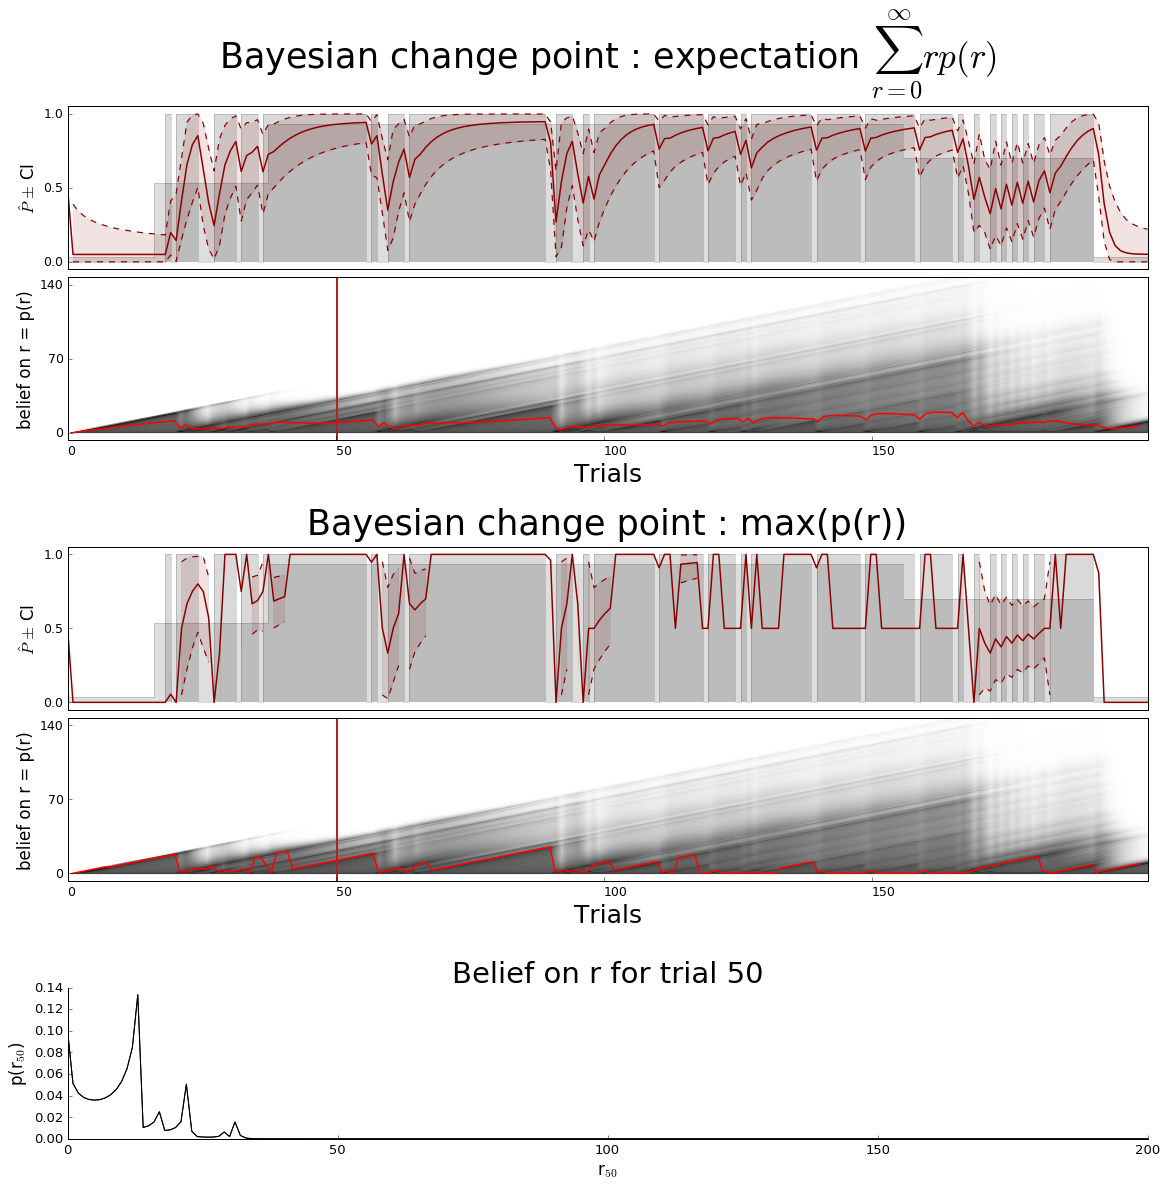
\includegraphics[width=0.2\linewidth]{bayesianchangepoint}};
	% cf 3_Results_2.ipynb ??
	\node [anchor=north west]  (img2) at (0.200\linewidth,.618\linewidth){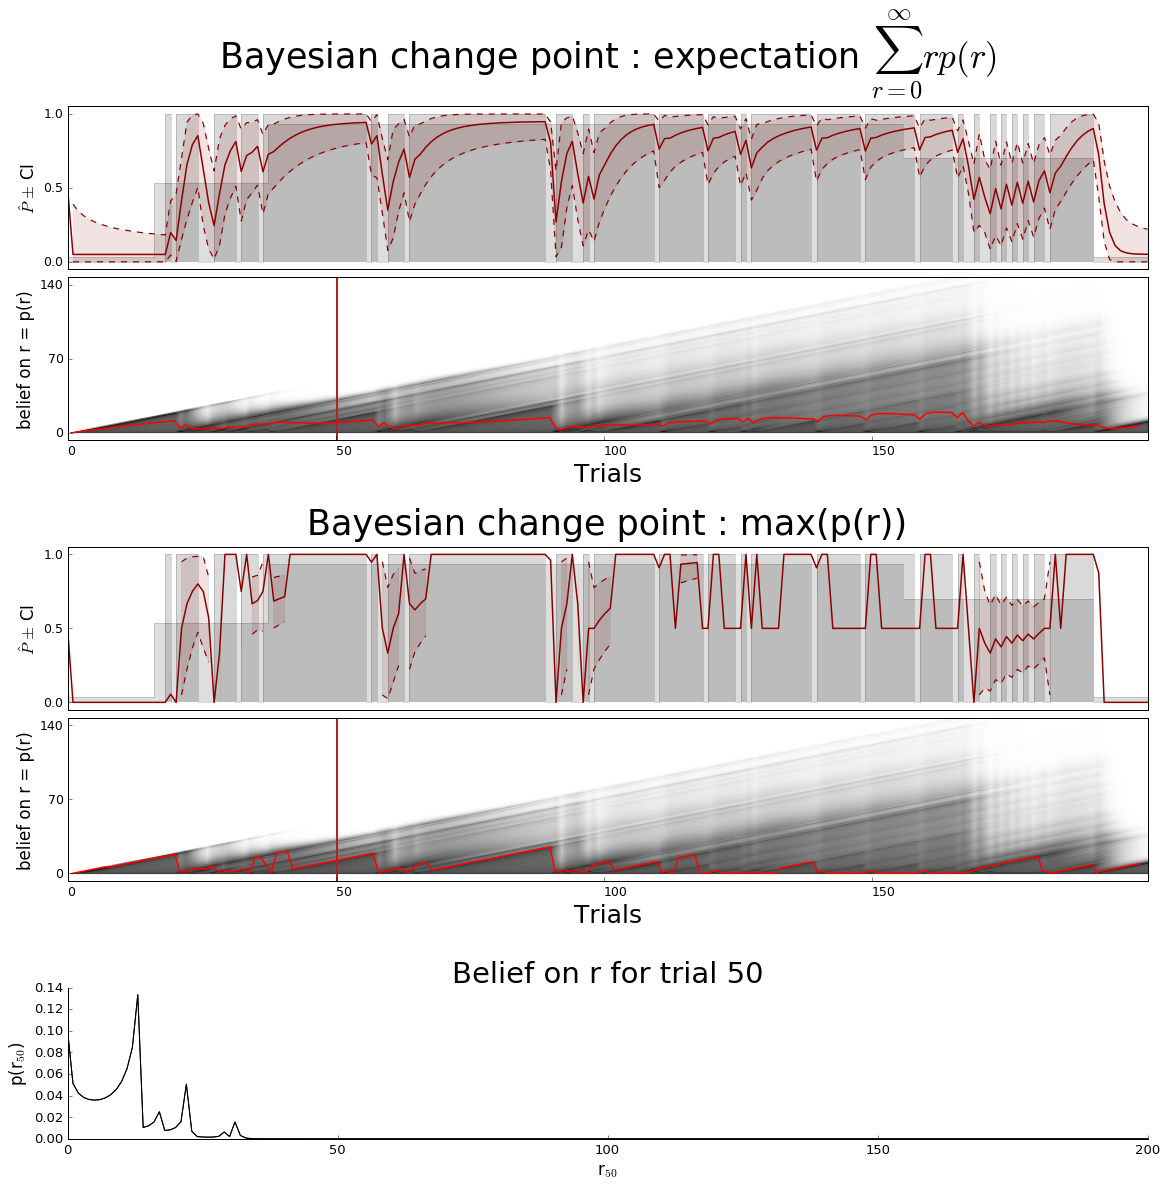
\includegraphics[width=0.8\linewidth]{bayesianchangepoint}};
	% cf 0_protocole.ipynb
	\draw [anchor=north west] (0.000\linewidth, .618\linewidth) node {$\mathsf{(A)}$};
	\draw [anchor=north west] (0.200\linewidth, .618\linewidth) node {$\mathsf{(B)}$};
\end{tikzpicture}
}	% cf 2_Methodes.ipynb ??
% ou cf 3_Results_2.ipynb
\caption{%
\emph{The binomial switching model and raw Psychophysical results}%
~\textbf{A}
This diagram represents the stochastic model chosen
to generate the sequence of directions.
It is represented as a graphical model representing
the three levels of the stochastic model. %
~\textbf{B}
%
% * I show here the overlay of this variable on the plot of
%  probability biases
%
% * these accelarations values were here scaled according
% to their extremal values.
%
% * there seems to be a trend with the polarity of the acceleration
% being negative for p values below .5 and positive for values above .5
%
% To observe the fit in an appropriate range between 0 and 1,
% the data for participant 18 was normalized and
% re-centered with the following transformation method:
% $\widetilde{aSPEM} = \frac{aSPEM_t-Min(aSPEM)}{Max_(aSPEM)-Min(aSPEM)}$.
%
Raw results for one characteristic observer.
In this plot we superpose the sequence of event
(red or black dots for respectively left or right directions),
the (hidden) evolution of the value of $p$ (horizontal black segments)
and the underlying times for switches (vertical black lines).
Note that we introduced pauses every  $50$ trials to prevent from fatigue.
% Each block is divided in 4 sub-blocks of $50$ trials as denoted by vertical black bars
Using a pseudo-random number generator with the same seed,
we could present the exact same sequence to all subjects. %
We have superposed the trace of
1/ the aSPEM strength as measured by the horizontal displacement
at the onset of the visually-driven SPEM (red line),
2/ the response to the bet experiment (red line) and
3/ the result of the BCP model (blue line)
along with the confidence interval for this estimate (blue shaded area).
}
\label{fig:results_raw}
\end{figure}
%-------------------------------------------------------------%
%: design of the binomial switching generative model
Indeed, to assess the dynamics of the adaptive processes
which compensate for the variability of sensory,
one may introduce a parametric mechanism controlling for its volatility.
By definition, volatility measures the temporal variability
of the sufficient parameters of a random variable.
In the HGF model~\citep{Matthys2011} for instance,
volatility is modeled as the non-linear transformation
of a random walk (modeled itself by a Brownian motion).
This models allows to generate a sequence of binary choices
where the variability fluctuates along a given trajectory.
Such a forward probabilistic model is invertible
using some simplifying assumptions and allows
to extract an inference of the agent's belief about volatility~\citep{Voessel??}.
Herein, we will use a simpler model where
The probability of this process varied in a piecewise-constant
(that is, a step function varying between~$0$ and~$1$),
similarly to~\citet{Meyniel13}.
For each trial, a target makes either to the left or to the right,
and we denote this variable as $x_0^t$ at trial $t$.
This direction being drawn from a Bernoulli process $\Bb$
with a parameter that we define as $p=x_1^t$.
The novelty is that this variable is chosen
at random from a prior distribution $\Pp$ at the moment of a switch.
The occurrence of these switches is itself drawn from a Bernoulli process
of probability $1/\lambda$.
Mathematically, this is easily described
by a graphical model~(\seeFig{results_psycho}-A) and
the following definition:
\eql{\choice{
x_0^t \eqdef o_t \propto \Bb(p^t) \\
x_1^t \eqdef p_t = p_{t-1} \quad \text{if} \quad s_t=0 \quad \text{and else} \quad p_t \propto \Jj \\
x_2^t \eqdef s_t \propto \Bb(1/\lambda)
}\label{eq:sgm}}.
Note that the prior distribution $\Pp$ can be for instance
the uniform distributions on $ [ O, 1 ] $ or
Jeffrey's prior~\seeApp{bcp}(TODO: put in appendix).
There is always a switch at $t=0$ and for each pause.
In conclusion, the experimental setup of the first session
is similar to that presented in~\seeFig{intro}-A, except for
this new generative model for the pseudo-random sequence of binary events
~\seeFig{results_psycho}-B.

%: outline
This paper is organized in five parts.
After this introduction, the next section will present
an inversion of the forward probabilistic model defined in~\seeEq{sgm}.
There is yet no such algorithm to our knowledge and
we will here provide with a solution
by extending previous results from~\citet{AdamsMackay2007}
to the case of binomial data.
We will also provide with a computational implementation
and a quantitative evaluation of this algorithm.
Then, we will present psychophysics on eye movements
to validate the generalization of previous results
In a first session, participants observe a target moving horizontally
with constant speed from the center
either to the right or left across trials~(\seeFig{intro}-A).
The probability of either motion direction changes randomly in time.
In a second session, participants are asked to estimate
"how much they are confident that
the target will move to the right or left in the next trial" and
to adjust the cursor's position on the screen accordingly~(\seeFig{intro}-C).
In the fourth part, we will analyze the inference of the volatility
for each individual participant.
This will allow the analysis of inter-individual changes for each session
and in particular in one could predict one's prior volatility,
that is, a measure of the dynamic compromise between exploration and exploitation
across the two different sessions testing predictive adaptive processes
at the unconscious and conscious levels.
Finally, we will summarize and conclude this study and
offer some perspectives for future work.
%: %%%%%%%%%%%%%%%%%%%%%%%%%%%%%%%%%%%%%%%%%%%%%%%%%%%%%%%%%%%%%%%
\section{Results: Bayesian change point model}

% These python scripts are available at \url{https://github.com/laurentperrinet/bayesianchangepoint}.
%TODO include changing point theory and bibliography
% TODO : check http://www.princeton.edu/~rcw2/papers/WilsonEtAl_PLOSCompBiol2013.pdf and bernouilli case + evaluation



See Matthys

Necessity of using a generative model


\subsection{Forgetful-agent model (Leaky integrator)}
% it's a particular case of the solution to the generative model assumaing a fixed -block length
%
% Following the~\citet{Maus2015} analysis, we performed a first study~page~\pageref{chap:4} in which we wanted to test a more realistic model of how trial-history shapes motion expectation in a direction-biased experiment.  According to~\citet{Anderson2006}, the temporal evolution for the expectation of a given event can be modeled making a simple assumption: the update of the estimated probability for an event is based on the discount of the previous estimated probability by a factor$~\lambda$, relative to new information. The value of$~\lambda$ presumably represents a compromise between responding rapidly to genuine changes in the environment and not prematurely discarding information still of value for slowly changing contexts. We extended~\citet{Anderson2006}'s approach to our analysis of anticipatory smooth pursuit across different contexts corresponding to the experimental blocks with different global probability-bias. We designed a forgetful agent estimating the target motion direction-bias according to the following iterative equation, where the estimated probability of a target moving rightwards is obtained from (1) the previous bias inference, (2) the imposed target directions and (3) a memory decay in the weighting of information. This model can be explained with the following equation:
%
%
%\[\hat{p}_{0} = 0.5\]
%\[\hat{p}_{i+1} = (1 - 1/\tau)*\hat{p}_{i} + 1/\tau * \textit{D}_{i}\]
%
%where
%\begin{enumerate}[label={}]
%\item $\hat{p}_{i}$ = estimation of rightward trials probability at trial~\textit{i}
%\item $\tau$ = characteristic memory decay time (in trials for the inference of $p$)
%\item $\textit{D}_{i}$ = Imposed directions. Sequence of 0 (leftward) and 1 (rightward) trials
%\end{enumerate}
%
% We simulated the sequence of p-estimates of the forgetful agent for each direction-bias block and for different values of~$\tau$. Fig~\ref{fig:p_est.pdf} below illustrates, for the $p=90\%$ direction bias block, the intuitive notion that with a small value for~$\tau$~(or equivalently a volatile memory) the agent's estimate is more sensitive to changes in the target direction trial sequence. On the other hand,  with larger~$\tau$~like 40 or 50, the estimation of p tends to fluctuate only very mildly around the global direction-bias over the experimental block.
%
%\begin{figure}[H]
%\centering
%\begin{subfigure}{1\textwidth}
%\includegraphics[width=1\textwidth]{p_est.pdf}
%\phantomcaption{\label{fig:p_est.pdf}}
%\end{subfigure}
%\caption[A forgetful-agent]{The forgetful agent's $p$-estimations with different values of~$\tau$ for the $p=90\%$ direction-bias block\label{fig:p_est.pdf}}
%\end{figure}
%
% Then, we performed a linear regression analysis of the relation between the experimentally measured anticipatory eye velocity and the simulated estimate of p for each direction-bias block. To do so, we again pooled together the eye movement velocity from all participants in each experimental condition and along the direction-bias estimated by the model at the time of their triggering. We then estimated the correlation coefficient $R$ as a function of~$\tau$. We found that $R$ is maximised for~$\tau = 5$ in $p = 50\%$ blocks ($R=.18$, $p<.05$) and $p = 75\%$ blocks ($R=.27$, $p<.05$) , and for~$\tau = 10$ for $p = 90\%$ blocks ($R=.32$, $p<.05$) (see Fig~\ref{fig:R_BL.pdf}). The correlation coefficient decreases for higher values of~$\tau$, coherent with the previous study from~\citet{Maus2015} from which we inspired this analysis. Still, the overall $R$ values are slightly higher compared to the raw linear regression with the unweighted fixed-size memory, indicating a better performance of this "forgetful" agent model.
%
%\begin{figure}[H]
%\centering
%\begin{subfigure}{1\textwidth}
%\includegraphics[width=1\textwidth]{R_BL.pdf}
%\phantomcaption{\label{fig:R_BL.pdf}}
%\end{subfigure}
%\caption[Pearson's R between experimental data and forgetful agent]{Linear regression coefficient R as a function of~$\tau$~$(1/\lambda)$ . This quantity is a rough estimate of the matching between the simulated p-estimates by the forgetful agent and experimental anticipatory eye velocity.\label{fig:R_BL.pdf}}
%\end{figure}
%
% We then looked at the linear relation of experimental data with the probability bias estimated by the model throughout all direction blocks for all our participants with~$\tau = 10$ and as we can see on Fig~\ref{fig:P_VEM_vs_pestBL.png}, we found a graded relation between Pearson's $R$ with  $R = .17$ ($p<.05$) in $p = 50\%$ blocks, $R=.27$ ($p<.05$) in $p = 75\%$ and $R=.30$ ($p<.05$) in $p = 90\%$ blocks. This shows that anticipatory smooth eye velocities are somehow related to the estimation of $p$ given by a forgetful agent. The overall computation of this analysis to all our condition showed, coherently with~\citep{Maus2015} (see study~\ref{chap:4},~page~\pageref{chap:4}), a tendency of having higher R's for short-memory, independently of the experimental condition (see Fig~\ref{fig:R_summary_2.pdf}). Though, it is important to note a better fitting quality for this using the forgetful-agent model as in~\citet{Anderson2006}.
%
%\begin{figure}[H]
%\centering
%\begin{subfigure}{1\textwidth}
%\includegraphics[width=1\textwidth]{P_VEM_vs_pestBL.png}
%\phantomcaption{\label{fig:P_VEM_vs_pestBL.png}}
%\end{subfigure}
%\caption[Anticipatory smooth velocity classified by the estimated probability bias]{Linear regression of anticipatory velocities in function of a~$\tau$~$(1/\lambda)$ = 10 estimation. \label{fig:P_VEM_vs_pestBL.png}}
%\end{figure}
%
%\begin{figure}[H]
%\centering
%\begin{subfigure}{1\textwidth}
%\includegraphics[width=1\textwidth]{R_summary_2.pdf}
%\phantomcaption{\label{fig:R_summary_2.pdf}}
%\end{subfigure}
%\caption[Relation between P-estimation and experimental conditions]{Linear regression of anticipatory velocities in function of a~$\tau$~$(1/\lambda)$ = 10 estimation for each conditions. \label{fig:R_summary_2.pdf}}
%\end{figure}
%
% To conclude on this section, the "forgetful agent" computed an exponentially-weighted moving average and estimated the probability of a stimulus going to the right given the previous instances of rightward stimulus and a progressive discount of past information. When we looked at the relation between aSPEM velocities and the direction-bias estimated by our model, we found higher Pearson's R for short-term memory ($\approx$ 5 to 10 trial history lengths) rather than long-term memory. However, a first critic could be that our proposed model may be too rigid and does not sufficiently imply the concepts of volatility~\citep{Behrens2007} or Bayesian uncertainty~\citep{Vilares2011}. It seems plausible that the memory (history length) the brain uses for inference is varying and that this variation could be related to the volatility inferred from information in the past. For instance, our model could not be applied to $p = 100\%$ rightward direction blocks because of a pretty quick saturation toward an estimation of probability equal to 1 even though experimental aSPEM datas shows a weak but existing proportion of aSPEM to the left direction. To address this hypothesis, our next model work will be inspired by a Bayesian Change-point detection model~\citep{Adams2007}, which mimics an ideal agent inferring both the likelihood of a specific event's occurrence with the volatility of the environment (e.g the duration since a change in bias).
%



\subsection{Bayesian change point model}

We have designed an agent adapted the Bayesian Online Change-point Detection model~\citep{AdamsMackay2007}. This model uses a latent variable r which represents the length of the current interval during which motion-direction probability ($\hat{P}$) has not changed. The agent infers at each trial the likelihood  of r and then deduces the optimal $\hat{P}$ (we used the expected value and the max as readouts) and the uncertainty associated to it. We simulated the model across our experimental sequences, as illustrated by the example for the third block.


%* an implementation of
%%[Adams &amp; MacKay 2007 "Bayesian Online Changepoint Detection"](http://arxiv.org/abs/0710.3742)
%in Python.
%
%````
%@TECHREPORT{ adams-mackay-2007,
%AUTHOR = "Ryan Prescott Adams and David J.C. MacKay",
%TITLE  = "Bayesian Online Changepoint Detection",
%INSTITUTION = "University of Cambridge",
%ADDRESS = "Cambridge, UK",
%YEAR = "2007",
%NOTE = "arXiv:0710.3742v1 [stat.ML]",
%URL = "http://arxiv.org/abs/0710.3742"
%}
%````
%
%* adapted from https://github.com/JackKelly/bayesianchangepoint by Jack Kelly (2013) for a binomial input.
%
%* This code is based on the  [MATLAB implementation](http://www.inference.phy.cam.ac.uk/rpa23/changepoint.php) provided by Ryan Adam. Was available at http://hips.seas.harvard.edu/content/bayesian-online-changepoint-detection
%
% * full code @ https://github.com/laurentperrinet/bayesianchangepoint


%-------------------------------------------------------------%
%:  FIGURE 3 fig:bayesianchangepoint
%: TODO présente le principe de l'algorithme, le résultat sur une séquence et une aanlyse quantitative qui permettra de l'utiliser pour les expériences psycho
\begin{figure}%[b!]
\begin{center}
% cf 3_Results_2.ipynb
    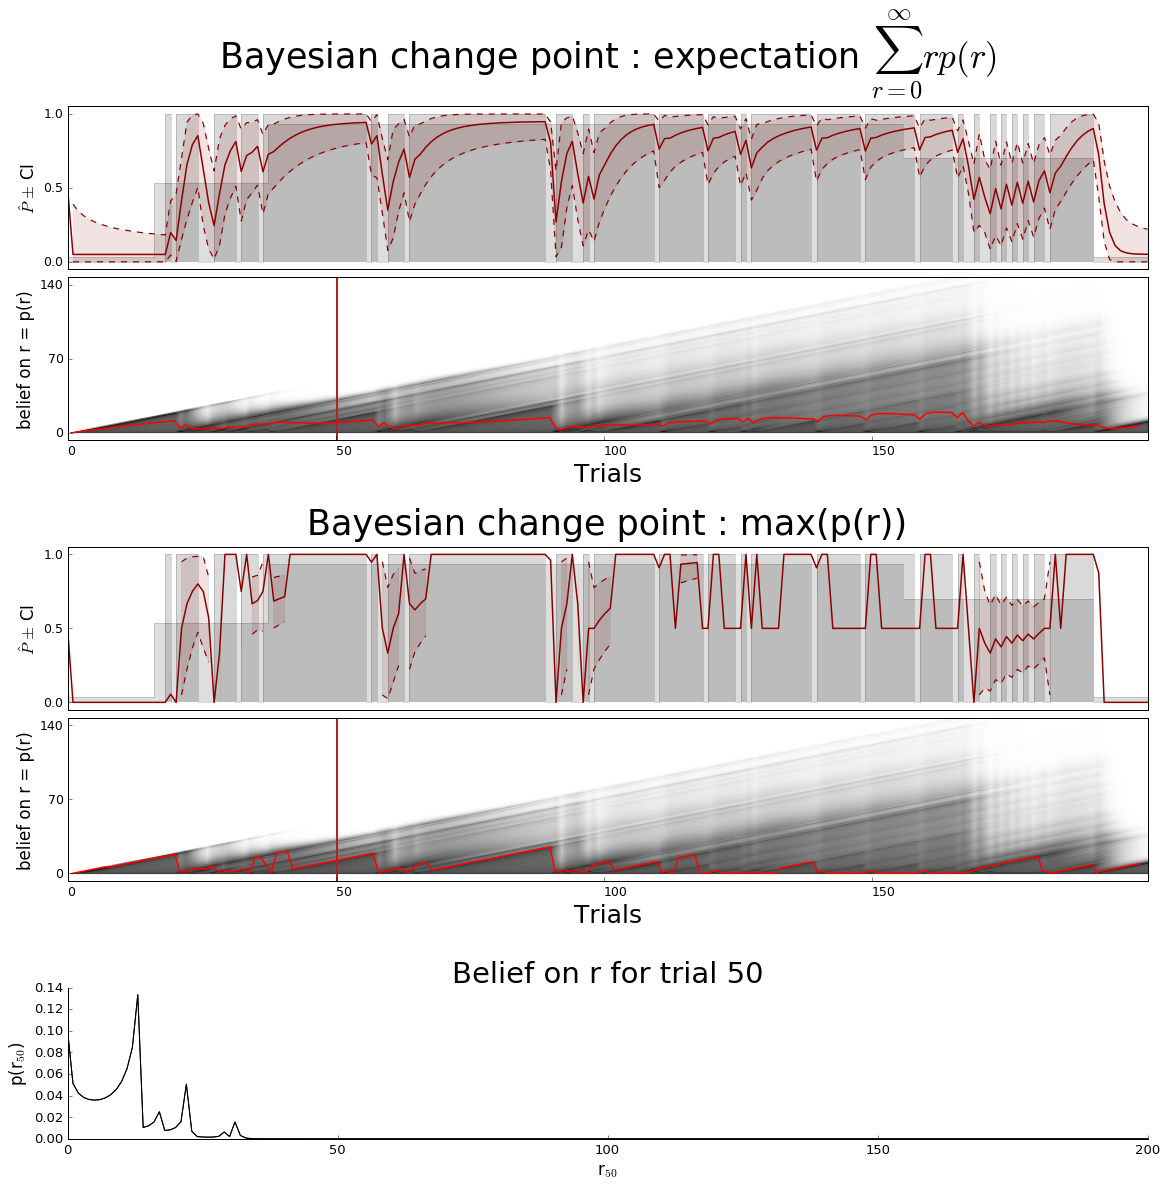
\includegraphics[width=1\linewidth]{bayesianchangepoint}
\end{center}
\caption{\emph{Bayesian change point model}~\textbf{A} shows hypothetic datas that works as a binomial choice, either 0 (leftward) or 1 (rightward). In particular, the probability switched at trials 6 and 10.~\textbf{B} shows the graph (treillis) on which the message indicates that mass probability is being passed. Black lines denotes "upwards", that is, for which there is a progression of the run length at the next step. The red line stands for the possibility that a switch happened, and then falls back to zero. The black curve stands for the run length of simulated datas in~\textbf{A} in function of time (r$_t$). We can see that the run length drops back to zero when change occurs at trials 6 and 10.
%\textbf{(C)}
%* in this graph information will be represented at different nodes. each node represent a belief which takes the form of a probability distribution over the set of parameters that we wish to describe.
%* it can be the mean and variance of a Gaussian, but in general it will be 2 parameters. in our case, we wish to estimate p (between zero and one) - it is characterized by the beta distribution (mathematically it is the conjugate of the bernouilli distribution)
%* (mathematically, we will use th family of exponenetial distributions:, gaussians, binomials) among which the beta distribution belongs
%First, we initialize the first node to prior values
%* at trial zero, there is no information, so we intiialize to the prior values
% use p log p + (1-p) log (1-p ) as in logistic regression?
}
\label{fig:bayesianchangepoint}
\end{figure}
%-------------------------------------------------------------%


Fig~\ref{fig:BCP_figA}~\textbf{A} shows one instance of a sequence of simulated datas of leftward and rightward trials with a probability $p$ of being rightward with possible variations through times. It also shows the predicted probability $\hat{p}$ by using the BCP algorithm. Fig~\ref{fig:BCP_figB} illustrates the belief r on the predicted probability $\hat{p}$ at a given trial. On Fig~\ref{fig:BCP_figC} and Fig~\ref{fig:BCP_figD}, we can see the belief on the run length estimation.

Note, the fixed-length is imply implemented by a (broken) line with fixed run-length $r_t=\tau$) - this allows for a simple comparison

\subsection{Bayesian change point algorithm}

%cf p33 de 2018-02-12 journal club bayesian changepoint chloe.pdf

% Fig~\ref{fig:BCP_figA}~\textbf{A} shows one instance of a sequence of simulated datas of leftward and rightward trials with a probability $p$ of being rightward with possible variations through times. It also shows the predicted probability $\hat{p}$ by using the BCP algorithm. Fig~\ref{fig:BCP_figB} illustrates the belief r on the predicted probability $\hat{p}$ at a given trial. On Fig~\ref{fig:BCP_figC} and Fig~\ref{fig:BCP_figD}, we can see the belief on the run length estimation.
%
%\begin{figure}[H]
%\centering
%\begin{subfigure}{1\textwidth}
%\includegraphics[width=1\textwidth]{BCP_fig.pdf}
%\phantomcaption{\label{fig:BCP_figA}}
%\end{subfigure}
%\begin{subfigure}{0\textwidth}
%\includegraphics[width=1\textwidth]{BCP_fig.pdf}
%\phantomcaption{\label{fig:BCP_figB}}
%\end{subfigure}
%\begin{subfigure}{0\textwidth}
%\includegraphics[width=1\textwidth]{BCP_fig.pdf}
%\phantomcaption{\label{fig:BCP_figC}}
%\end{subfigure}
%\begin{subfigure}{0\textwidth}
%\includegraphics[width=1\textwidth]{BCP_fig.pdf}
%\phantomcaption{\label{fig:BCP_figD}}
%\end{subfigure}
%\caption[Bayesian Change Point model computation]{~\textbf{A} is a sequence of points representing leftward (0) of rightward trials (1) with a given probability $p$ of being rightward and that changes at some trials (clear red). The predicted probability $\hat{p}$ ($\tau=N_{trial}/4$ tells the BCP that the probability is more susceptible to change every $N_{trial}/4$), continue and dotted dark red lines shows the $p$$-$estimation.~\textbf{B} shows the probability of the run length, the probability of the having same probability consecutive trials. The red line represents the $\hat{r}$, that represents the sum of he products of each r (number of consecutive trials having the same probability)  $\sum_{r=0}^\infty r \cdot P(r)$.~\textbf{C} represent the probability of each r for trials 50 and 250 along their $\hat{r}$ and their $\hat{p}$. For instance, for trial 50, we can observe that $\hat{r}$ is close from the real number of trials during the probability has not change (real $p$ stayed for 50 trials). $\hat{p}$ is also pretty close from the real $p$ ($p=1$).~\textbf{D} shows that at trial 250 $\hat{r}$ is more far than the real r that is also equal to 50 trials. But here, $\hat{p}$ is closer from $p$ that is equal to 0.75. \label{fig:BCP_fig.pdf}}
%\end{figure}
%
% We adapted this model to the data our first study,~page~\pageref{chap:4}, by taking the alternating output of leftward/rightward trials as the sequence of observations that will be under the analysis of the model. This model uses a latent variable r which represents the length of the current interval during which motion$-$direction probability~($\hat{p}$)~has not changed. The agent infers at each trial the likelihood of r and then deduces the optimal~$\hat{p}$~(we used the expected value and the max as readouts) and the uncertainty associated to it. Finally, the whole algorithm simplifies to the following iterations:

Following the principle of Active Inference,
To summarize, the algorithm % uncover progressively

\begin{enumerate}
	\item     Initialize

	\begin{itemize}
		\item    $P(r_0)= S(r)$ or $P(r_0=0)=1$ and
		\item    $\nu^{(0)}1 = \nu_{prior}$ and $\chi^{(0)}1 = \chi_{prior}$
	\end{itemize}

	\item    Observe New Datum $x_t$
    \item    Evaluate Predictive Probability $\pi_{1:t} = P(x |\nu^{(r)}_t,\chi^{(r)}_t)$
    \item    Calculate Growth Probabilities $P(r_t=r_{t-1}+1, x_{1:t}) = P(r_{t-1}, x_{1:t-1}) \pi^{(r)}_t (1-H(r^{(r)}_{t-1}))$
    \item    Calculate Changepoint Probabilities $P(r_t=0, x_{1:t})= \sum_{r_{t-1}} P(r_{t-1}, x_{1:t-1}) \pi^{(r)}_t \cdot H(r^{(r)}_{t-1})$
    \item    Calculate Evidence $P(x_{1:t}) = \sum_{r_{t-1}} P (r_t, x_{1:t})$
    \item    Determine Run Length Distribution $P (r_t | x_{1:t}) = P (r_t, x_{1:t})/P (x_{1:t}) $
    \item    Update Sufficient Statistics :
	\begin{itemize}
		\item    $\nu^{(0)}_{t+1} = \nu_{prior}$, $\chi^{(0)}_{t+1} = \chi_{prior}$
		\item    $\nu^{(r+1)}_{t+1} = \nu^{(r)}_{t} +1$, $\chi^{(r+1)}_{t+1} = \chi^{(r)}_{t} + u(x_t)$
	\end{itemize}

    \item    Perform Prediction $P (x_{t+1} | x_{1:t}) = P (x_{t+1}|x_{1:t} , r_t) P (r_t|x_{1:t})$
    \item    go to (2)
\end{enumerate}


where $\KL{\hat p}{p}$ is the Kullback-Leibler divergence between samples $\hat p$ and model $p$ under a Bernouilli distribution
\begin{equation}
\KL{\hat p}{p} = \hat{p} \log\pa{\frac{\hat p}{p}} + (1-\hat p) \log\pa{\frac{1-\hat p}{1-p}}.
\end{equation}


Contrary to the forgetful-agent model where~$\tau$ was a fixed parameter, the BCP use a changing~$\tau$ parameter. In the latter the~$\tau$ parameter informs the BCP model that the probability is suspected to change every~$\tau$ trials. As we can see on~\ref{fig:search_tau.png}, participants do not have the same pattern of responses (examples of participants 16 and 18 below). Still we were able to extract the parameter~$\tau$ that maximizes the fit between the probability computed by the BCP model ($\hat{p}$) and the experimental datas.

%\begin{figure}[H]
%\centering
%\begin{subfigure}{1\textwidth}
%\includegraphics[width=1\textwidth]{search_tau.png}
%\phantomcaption{\label{fig:search_tau.png}}
%\end{subfigure}
%\caption[Correlation maximization in function of  $\hat{p}$ in the BCP model]{This figure shows the evolution of the correlation between $\hat{p}$ and the experimental datas of participants 18 and 16 in function of~$\tau$ (i.e the point where $p$ is suspected to change) for each experimental condition and probability block (color-coded, see legend). Points represent the~$\tau$ that maximizes the correlation between datas and $\hat{p}$ in our different modalities
%\label{fig:search_tau.png}}
%\end{figure}

\hfill \break
 Then we looked at the fit between the probability predicted by the BCP $\hat{p}$ (for the sequences of events (rightward and leftward trials) that we used for our different experimental blocks) and the experimental datas obtained by participants. As we can see on fig~\ref{fig:data_fit_S18.pdf} we have a nice fit between the normalized aSPEM behavioral datas of participant 18 and the probability~$\hat{p}$ computed by the BCP.



%\subsection{Computing the likelihood}
The main difference between our algorithm and that of Wilson is the way that the likelihood is computed.
%different read-outs : see 2018-02-12 journal club bayesian changepoint chloe.pdf p.33

See also Radillo / Brady 2017 - Rats and dyncmac envt - allows to extend to the continuous case

\subsection{Quantitative analysis of the Bayesian change point algorithm}
we see that as in the synthetic example above,
there is a correct detection of switch after a short delay of a few trials

in particular, from this correct detection,
the value of the inferred probability approaches
the true one as the number of observations increase in one subblock.

again, we see that a fixed length model gives a similar output
but with the two disadvantages described above


%different read-outs : see 2018-02-12 journal club bayesian changepoint chloe.pdf p.42
Let's now see the application of our model to a simple synthetic example before applying it to the experimental protocol that we used in our two experiments


- we show two panels, one below which displays the value of the belief for the different run-length, and one above where we will show the resaulting prediction of the next outcome.
we obtain for any given sequence different values at the given trial in the form of columns for any possible run-length: the belief,
and the sufficient statistics for the beta distirbution which allow to provide with an estimate of the current probability

- first, we show the value of probability, low probabilities are blueish while high probabilities. at every trial, the agent evluates the value for the different possible run lengths, generating a column. by showing all columns we generate this image which shows the evaluation along the sequence of trials.

- second we show above the sequence of observations that were shown to the agent in a light black line. the read line gives an evaluation of the most probable a posteriori probability as the probability to hte run-length the maximum a posteriori belief on the differettn beliefs about run-lengths. using the estimate of the precision at this

We remark two main observations:

- first, beliefs grow at the beginning along a linear ridge, as we begin our model by assuming there was a switch at time 0. Then we observe that at a switch (hidden to the model), the model
such that belief is more stronlgly diffused until the probability

-second, we may use this information to read-out the information the most probable probability and the confidence interval as shown by the red dashed lines (.05, and .95)


This is in contrast with a fixed length model, for which
- the delay will always be similar
- there is no dynamic upDATE OF THE INFERRD probability


as a summary, for any given sequence,
 we get an estimate of the probability given by the ideal observer.
 we will now see how we can apply that to our experimental protocol.
 We expect it to be harder than the previous protocol
 in fixed-length blocks

%: %%%%%%%%%%%%%%%%%%%%%%%%%%%%%%%%%%%%%%%%%%%%%%%%%%%%%%%%%%%%%%%
\section{Results: psychophysics}
%%%%%%%%%%%%%%%%%%%%%%%%%%%%%%%%%%%%%%%%%%%%%%%%%%%%%%%%%%%%%%%
%%%%%%%%%%%%%%%%%%%%%%%%%%%%%%%%%%%%%%%%%%%%%%%%%%%%%%%%%%%%%%%
\subsection{Eye movements recordings}
%%%%%%%%%%%%%%%%%%%%%%%%%%%%%%%%%%%%%%%%%%%%%%%%%%%%%%%%%%%%%%%
%: raw results show a qualitative trend
We applied the binomial switching model
to generate the (pseudo-)random sequence of
the dot's directions,
and in a first session, we recorded the participants' eye movements.
Among our $12$ subjects,
we show one representative example in~\seeFig{results_raw}-B.
This representative participant was chosen as that
with the median fit in the quantitative analysis
that will follow (\seeSec{inter}).
In particular, we superposed over the actual sequence of binary choices
(leftward or rightward - respectively red or black dots)
the true value of the true (hidden) value
of the binomial process (horizontal black segments).
In general, results are more variable when the bias is weak ($p\approx .5$)
than when it is strong (close to zero or one),
consitent with the dependence of the variance of the binomial process
as a function of the probabilistic bias ($p$).
Let's now see how this applies to our experimental results
by comparing human observers to our bayesian agent.
More interestingly, we also superposed
the observed value of the strength of aSPEM
(the total velocity VEM, red line)
the value of the readout inferred probability
(as a blue line, along with its confidence interval in a shaded area).
Comparing the raw eye movement results with the latter,
it seems qualitatively that both traces evolve with a good fit.
First, both have similar delays in detecting a switch,
reflecting the time (of the order a few trials) taken to integrate enough information
to switch to a novel probability bias value in the binomial process.
Second, the precision (that is, the inverse of the variancve)
of the inferred probability $\hat{p}$ seems to increase
in bigger sub-blocks as information is integrated over more trials.
As a result, the inferred probability as a function of time
seems qualitatively to constitute a useful regressor
with the strength of aSPEM.

%-------------------------------------------------------------%
%: FIGURE 4  fig:results_psycho \seeFig{results_psycho}
\begin{figure}%[b!]
% cf 3_Results_2.ipynb
\begin{center}
    \includegraphics[width=1\linewidth]{results_KDE_VEM_vs_p_hat}
    \includegraphics[width=1\linewidth]{results_KDE_bet_vs_p_hat}
\end{center}
\caption{\emph{Psychophysical results over all participants}
Each trial in our experimental results in an estimate of
the strength of aSPEM (as measured by VEM)
and a rating scale value.
Relating those values with the corresponding inferred value $\hat{p}$
of the probability bias,
this constitutes a scatter of values.
We display these relationships using a
Kernel Density Estimation (KDE) of the relationship between $p$ (abscissa)
and \textbf{(A)} VEM and \textbf{(B)} the value of bet (in ordinates).
In \textbf{(A)}, we have overlaid is a regression line which shows
a high correlation factor ($R=XXX$) which is superior to that found
with the fixed-length design (see Appendix ...)
but also with other models described in the text
(fixed-length estimator, maximum BCP - see Appendix ... ).
In \textbf{(B)}, we have fitted the data with a logistic regression
showing a negligeable intercept (no bias) linked to the symmetry
of the problem, but a consistent slope showing an aversion to risk
(cf Kanehman).
%\textbf{(C)}
}
\label{fig:results_psycho}
\end{figure}
%%-------------------------------------------------------------%
%: quantitive analysis
Quantitatively, we wanted to look at the quality of fit
between the strength of aSPEM and
the probability $\hat{p}$ computed by the BCP algorithm.
In~\seeFig{results_psycho}-A, we have plotted for all subjects
this strength as a function of the inferred probability
that was coded at the second layer and which is unknown to the observer.
% TODO: First, the trend that we put in evidence is the identity of the observer
As we can see in~\seeFig{results_psycho}-A,
the probability $\hat{p}$ computed by the BCP algorithm
has a positive linear relationship with the aSPEM velocity.
Note that since the BCP is a probabilistic model,
we can also compute the Mutual Information and
compare that value with that obtained by other models~\seeApp{bcp}.
The corresponding Pearson correlatio coefficient
is slightly higer than that found in
the classical experiment with fixed blocks~\seeFig{intro}-B.
This is surprising at a first sight as the blocks are of random length,
and that participants have to adapt to such a volatile environment.
However, when faced with some new observations,
the observer has to constantly adapt his response
to either exploit this information by considering that
this observation belongs to the same sub-block or to explore
a novel hypothesis.
This compromise is one of the crucial component that we wish to explore
and which is well captured by the BCP model.
In particular, the model predicts the different facets
from the experimental results,
from the variability as a function of the inferred probability,
to the dynamics of the bahaviour following a (hidden) switch.
As a consequence this provides with a stronger correlation,
as measured by the Pearson coefficient.
We deduce that the trace of inferred probabilities is a powerful regressor
to explain the strength of aSPEM.
We will now try to extend this result
to the second session with rating scales.
%%%%%%%%%%%%%%%%%%%%%%%%%%%%%%%%%%%%%%%%%%%%%%%%%%%%%%%%%%%%%%%
\subsection{Rating scale recordings}
%%%%%%%%%%%%%%%%%%%%%%%%%%%%%%%%%%%%%%%%%%%%%%%%%%%%%%%%%%%%%%%
%: qualitative analysis \seeFig{results_psycho}-B
As we could assess qualitatively in~\seeFig{results_raw}-B,
the trace of the rating scale seems to correlate well
with the inferred probability $\hat{p}$.
Similarly to the strength of aSPEM,
(1) this traces exhibits also a positive correlation
(the next outcome will in general be correctly inferred,
as compared to a random choice),
(2) stronger biases lead to lower variabilities in the estimate,
(3) a (hidden) switch in the value of the bias is
most of the time correctly idetified after only a few trials.
Note also that at every pause (black vertical bar),
participants tended to provides with more neutral scales
than at the end of a sub-block of trials.
This would correspond to a resetting mechanism
of the predicted value of the next outcome.
As a consequence, the experiment performed in the second session
shows that the value that is consciously evaluated by participants
are qualitatively similar to that which is unconsciously generated behaviourally
in the form of the strength of aSPEM.

%: quantitative analysis
Similarly to~\seeFig{results_psycho}-A,
we now compare quantitatively the value of rating scale
as measured during the second session.
The KDE estimate shown in~\seeFig{results_psycho}-B,
represents the reliationship between
the estimated proability
and the value which was predicted at each trial
by participants for the outcome of the next trial.
This exhibits a consistant relationship
but which now follows a non-linear trace.
In particular, this relationship was finer
in comparison with a other agents
such as the forgetful agent~\seeApp{results_psycho}
We modelled this behaviour as
a logistic regression over
the log-odd ratio estimated by the agent.
This analysis provide with regression factors for each participant. %TODO
It shows that the bias (intercept)
was negligeable, while the slope (logistic factor)
was always positive.
This indicates a generic aversion to risk~\citep{KanehmanXX}
such that the value of a possible outcome
is down-weighted by the precision of the inferrence.
Our logistic regression analyses
suggests that this may come from a multiplicative weight
on the (log-) odd-ratio which is chosen as a rating scaled
compared to the (log-)odd-ratio of the inferred probability.

\subsection{Analyzing inter-individual differences}
\label{sec:inter}

representative example in~\seeFig{results_raw}

with time characteristics $\tau$

By extracting the parameters for every subject
we can expect to characterise inter individual differences.

%-------------------------------------------------------------%
%: FIGURE 5  fig:results_inter \seeFig{results_inter}
% TODO présente une meta analyse qui montre une correlation par sujet (scatter plot) entre h_a et h_bet (see 2017-11-16 chloe figures.pdf ) y-a-til un continuum entre explorateurs et conservatezurs?, voir de montrer une causalité entre les 2 expériences - on pourrait superposer aussi les résultats si on avait utilisé un fixed-length ?
\begin{figure}%[b!]
\begin{center}
    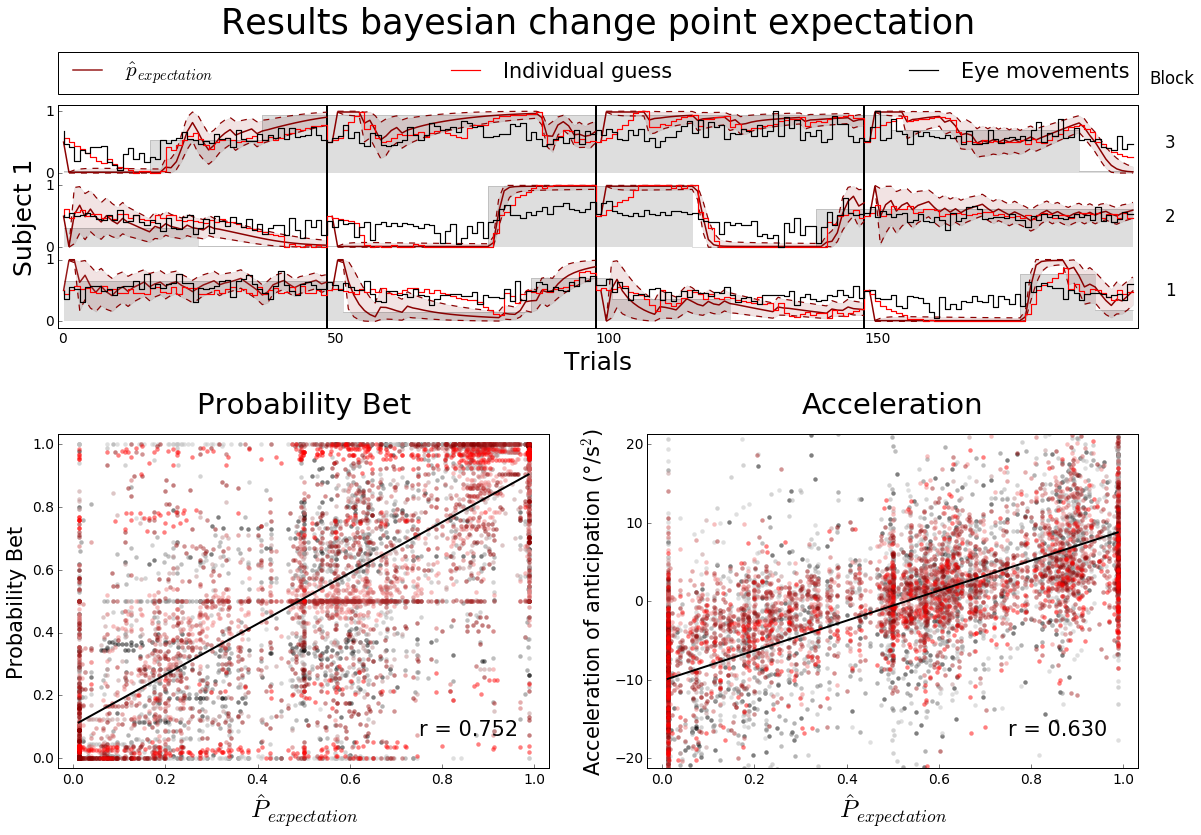
\includegraphics[width=1\linewidth]{results_bayesianchangepoint_e}
\end{center}
\caption{\emph{Analyzing inter-individual differences} \textbf{(A)}
\textbf{(B)}
\textbf{(C)}  }
\label{fig:results_inter}
\end{figure}
%-------------------------------------------------------------%

There are a spectrum of individual choices
between exploration and exploiting behaviors.


%: %%%%%%%%%%%%%%%%%%%%%%%%%%%%%%%%%%%%%%%%%%%%%%%%%%%%%%%%%%%%%%%

\section{Discussion}


%The oculomotor system has to constantly update its knowledge about the environment. An ordeal is then to adapt to changes with the shortest delays. Early studies have proposed that stimuli provides information to modulate reaction times within sequences~\citep{Hyman1953, Tune1964, Schvaneveldt}. This theoretical approach is coherent with the notion of local transition probabilities that quantifies at which extent an observation deviates from the preceding ones~\citep{Meyniel2016}. The way expectations act on cognitive processes has been investigated by a wide range of domains such as predictive coding~\citep{Wolpert2000, Wacongne2012}, active inference~\citep{Friston2010}, motor control~\citep{Sutton1998, Behrens2007} and reinforcement learning~\citep{Nassar2012}. Non-stationary observations can also explain why both local and global effects emerge and why local effects persist in the long run even within purely random sequences~\citep{Cho2002, Yu2009}. This constant update of a general belief on the world can be a consequence of the constant attempt to learn the non-stationary structure of the environment that can change at unpredictable times~\citep{Yu2009}. Many studies have actually already pointed the brain's ability to apprehend non-stationary states in environments~\citep{Ossmy2013, Meyniel2015}. As explained by~\citet{Meyniel2016}, the belief upon an environment can be divided in two different ways:
%
%\begin{enumerate}[label=\Alph*)]
%\item Update the~\textit{a priori} likelihood of a sudden change, also known as the volatility and taken into account by the model~\citep{Behrens2007}
%\item A leaky integrator factor imbedded in the model~\citep{Anderson2006, Yu2009, Ossmy2013, Wang2002}
%\end{enumerate}
%

%: theory / computationnally-driven experiments
% it's a main novelty
genrative models for changing environments allows to know the ground truth compared to natural stimulation (see Rust eand Movshon)%
Let's remember our hierarchical generative model.

At any given trial, we wish to construct an algorithm which

We will introduce a fundamental component of Bayesian models : a latent variable

this new variable will be used to test different hypothesis which will be evaluated to predict future states. it is called latent because it aims at representing a variable that is latent (or hidden) to the observer

in our case, we will assume that the bayesian model knows about the structure of the generative model and we will set it to the current run-length $r$, that is, at any given trial, the hypothesis that the past r observations belong to the same block. of course a wrong choice of a latent variables (let's say the temperture in the experimental room) may give unexpected results, even is the bayesian model is "optimal" - an essential point to understand in bayesian inference

extension to multi-nomioal( daniele + fred danion)



% Still, only Bayesian models recover an explicit probabilistic representation of change in likelihood. Recent experimental studies suggest, indeed, that the brain is able of estimating a hierarchical model of the environment and that humans can explicitly report sudden changes in sequences~\citep{Meyniel2015, Gallistel2014}. Ultimately, we passed over one of leaky integrator models' main default, having a too fixed and rigid memory parameter. In our work the memory parameter is constantly inferred by the BCP algorithm over the observation of the number of trials where this inference stayed reliable and then globally represented probabilistic representation of changes in likelihood and actualization of~\textit{a priori} knowledge.


perspectives:
- RL : use hindsight example of localization for saccades: get the changepoints then improve estimate of reward allows to optimize the association between the set of measures and their utility (compared to Q-learning where it is a fixed length)
- interindividual differences : markers for the berhaviour traces - traces of the network implementation
- the brain is weakly Bayesian (it does not care about equations but more about sugar)


%: %%%%%%%%%%%%%%%%%%%%%%%%%%%%%%%%%%%%%%%%%%%%%%%%%%%%%%%%%%%%%%%

\section{Conclusions}


\begin{itemize}\setlength{\itemsep}{0ex}
\item There is a strong correlation between the real probability and the value of the bet,

\item there is a stong correlation between the strength of anticipation and the probability of the process,

\item we have developed a Bayesian model of an agent estimating the probability of changing points. This allows to dynamically infer the direction probability and directly compare model and human behaviour.

% to summarize, we have shown that
% - there is a correlation in the anticiapatory response of eye movements
% in a volatile environment that is captured if we know the true probability
% - that a fixed length models captures some of this correlation, but that
% - our online bayesian changep[oint model better captures this correlation
% and that this may hint at the neural mechanisms used to anticipate
% in a dynamic environment
%
% the brain is not strongly a bayesian machine, but weakly

\end{itemize}
%: %%%%%%%%%%%%%%%%%%%%%%%%%%%%%%%%%%%%%%%%%%%%%%%%%%%%%%%%%%%%%%%
\section{Material and Method}
%%%%%%%%%%%%%%%%%%%%%%%%%%%%%%%%
%%%%%%%%%%%%%%%%%%%%%%%%%%%%%%%%
\subsection{Psychophysics}
%%%%%%%%%%%%%%%%%%%%%%%%%%%%%%%%



% TODO replace this with the actual protocol using psychopy

%cf. https://github.com/chloepasturel/AnticipatorySPEM/issues/19
\textbf{Stimuli were generated using PsychoPy 1.85.4 on a Mac running OS 10.6.8 (A VERIFIER) and displayed on a 20" Viewsonic p227f monitor (A VERIFIER) with resolution $1280\times 1024$ at 100~\si{\Hz} (60 ?). Psychophysics routines were written using PsychoPy 1.85.4 controlled the stimulus display. Observers sat 57~\si{\cm} from the screen in a dark room. Twelve observers (29 years old +/- 5.15) with normal or corrected-to-normal vision took part in these experiments. They gave their informed consent and the experiments received ethical approval from the Aix-Marseille Ethics Committee in accordance with the declaration of Helsinki.}
%Stimuli were presented on a 21 inches CRT monitor with refresh rate of 100 Hz. Stimuli were generated using the Psychophysics Toolbox extension for Matlab (Brainard, 1997; Pelli, 1997) running on a Mac Pro (first generation) computer and displayed at a viewing distance of 57 cm against a gray background. The luminance of the gray background was 42 cd/m2. To minimize measurement errors, the subject’s head movements were restrained using a chin and forehead rest, so that the eyes in primary gaze position were directed towards the center of the screen. Eye movements were measured continuously with an eye tracking system (Eyelink 1000, SR Research Ltd., sampled at 1000 Hz) and data were transferred, stored, and analyzed offline using programs written in Matlab or Ipython notebooks.
%Recorded horizontal and vertical gaze position were low-pass filtered using a Butterworth (acausal) filter of order 2 with a 30 Hz cut-off frequency and then were numerically differentiated to obtain velocity measures. We used an automatic conjoint acceleration and velocity threshold method to detect saccades (Krauzlis & Miles, 1996) and further inspected all individual traces visually to exclude aberrant trials. Saccades were excluded from eye velocity traces (and replaced by NaN values in the numerical arrays) before trial averaging. We evaluated the effects of the experimental manipulations on anticipatory velocity at the individual level, by comparing the mean eye velocity during a critical time window, between –50 and +50ms around target motion onset (as highlighted in Figure 2), using individual one-way ANOVAs (with the probability bias or reinforcement type as 3-levels single factors). We also computed all post-hoc pair-wise comparisons using Tukey’s HSD test. Even though the normality assumption of our data was fairly justified given the sample’s size (always over 60 trials per condition), we also computed non-parametric statistics (Kruskal-Wallis test) for comparison and results were similar. All tests and analyses have been realized using Python 3.5 with the Numpy and Scipy libraries.
3 blocks of 200 trial - with 4 sub-blocks of 50 trials


 * the whole experiment was coded by Chloé using :
 - python for the generative model,
 - the psychopy library for the stimulus display + connection to the eyelink 1000 that we used to record EMs
 - numpy, pandas and pylab for the data analysis

  * all this code is available : for running the experiments, re-analyzing the data and doing all plots are on github

These python scripts are available at \url{https://github.com/chloepasturel/AnticipatorySPEM}.


We asked subjects to perform two tasks on different days :
%\begin{itemize}\setlength{\itemsep}{0ex}
%\item a <<Bet>>
%\item a <<recording>>
%\end{itemize}

In summary, the design of our experimental setting is therefore very similar to the previous experiment but with a more general construct:

- using the same 3-layered generative model, we generated sequences of directions

- and generated 3 blocks of 200 trials

- with an average block length of 40 trials

We anticipated that such an  experiment for which we simply recordedd the eye movements should be more difficult for observers compared to the classical experiments with longer (400 trials), fixed blocks and...

\subsection{The Bet}
In this first part, the subjects must simply answer before each trial at the question \textit{ ``How sure are you that the target will go left or right''}. This was performed by adjusting a cursor on the screen using the mouse (see Figure).

%\textbf{ Un point de fixation blanc de 10px de large est affiché au début d'un essai. Les sujets doivent ajuster le curseur sur une échelle blanche gradué placé en desous. Cette échelle présente 3 graduations : 'gauche' et 'droite' au extrémité et 'incertain' au millieu. Pour validé leurs choix, les sujets doivent cliquer sur la souris. L’échelle et le point de fixation disparaissent et une cible en mouvement à 15°/s (voir pour LB$_Bet$ 20°/s) s’affiche à l’écran. La cible est un cercle blanc mesurant 10px de large et 2px de lineWidth.}


%\textbf{Lors de cette tâche les mouvement oculaire sont enregistré à 100 Hz via Eyelink 100. Le module Python Pylink (SR research) 0.1.0 nous a permis de faire le lien entre Eyelink et nos routines python. Les sujets ont la tête fixe, et on leur demande de ne pas cligner des yeux lorsque le stimuli aparait. Chaque essais commence par la présentation d’un point de fixation blanc de 10px de large au centre de l’écran pendant une durée variable de 400 à 800 ms. Si le signal enregistré n'est pas présent dans une fenêtre de $120\times 120$ px autour du point de fixation ou si il n’est pas stable (clignement, mauvais enregistrement…), la durée de fixation recommence. À la fin de cette durée de fixation il y a un GAP de 300ms, le point de fixation disparait laissant juste un écran gris. Puis une cible en mouvement de 15°/s apparaissait de sorte que 100ms après sont apparition il soit au centre de l’écran, afin d’évité la première saccade. La cible est un cercle blanc mesurant 10px de large et 2px de lineWidth (REDONDANT).}


This is why we added a supplementary experiment for each observer but on a different day for which we asked at every trial to give a subjective, conscious evaluation of the direction of the next trial + a confidence about this inference. Once this information given by the subject, we were showing the actual outcome.

Interestingly, we used exactly the same sequence, allowing to make a direct comparison of the results of both experiments

We called this experiment the bet experiment.


\textbf{Tous les 50 essais le 'score' du sujet sur les 50 derniers essais est affiché au centre de l'écran, le sujet doit appuyer sur la barre espace du clavier pour continuer (doit dire a l'expérimentateur quand il veux continué, on ne pouvais pas brancher une souris et un clavier en même temps). Ce score est égal à $\sum_{x=0}^{50} \frac{Bet_{x} \times dir_x}{50} \times 100$. Où $Bet_x$ est le parie du sujet à chaque début d'essaie comprie entre -1 pour la gauche et 1 pour la droite, $dir_x$ est la direction de la cible pour chaque essai, -1 pour la gauche et 1 pour la droite.}


%\subsection{The Bet}
%Example of results obtained during the bet :
%\begin{center}
%    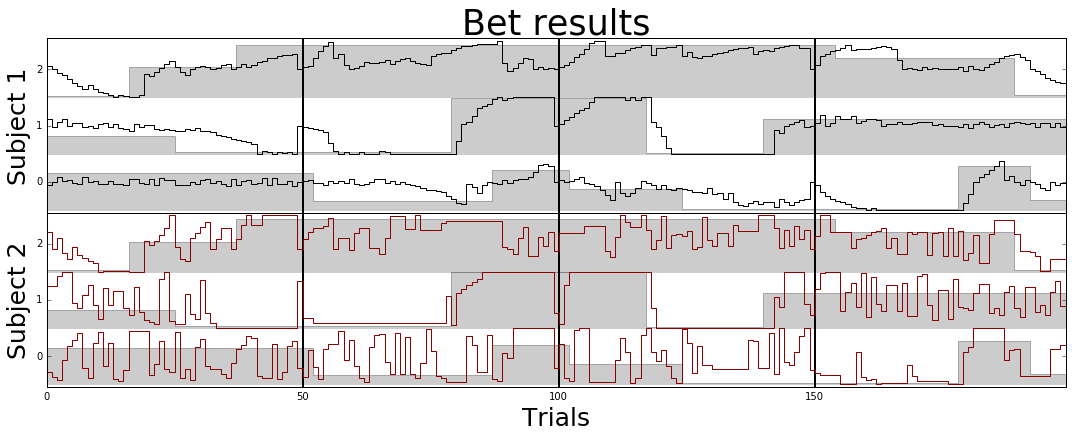
\includegraphics[width=1\linewidth]{results_pari}
%\end{center}
%%Comparison of probabilities bet with respect to the real probability :
%The scatter plot of the value of the bet (probability bet) as a function of the real probability at every given trial shows that there is a good correlation between both values:

%\begin{center}
%    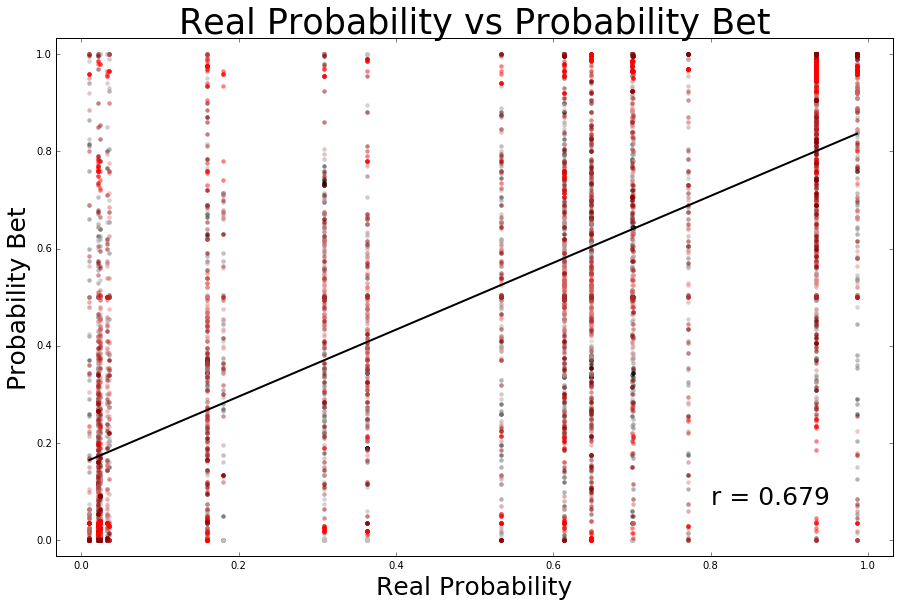
\includegraphics[width=1\linewidth]{p_real--p_bet}
%\end{center}

\subsection{Eye movements recording}

%
%Experiment 1: motion direction-bias task (Baseline)
%	 The visual stimulus used in experiment 1 was a white ring (0.30° outer diameter and 0.23° inner diameter) with a luminance of 102 cd/m2 that moved horizontally on a grey background. Each trial started with a central fixation point displayed for a random duration drawn from a uniform distribution ranging between 300 and 600ms. Then a fixed-duration 300ms gap occurred between the offset of the fixation point and the onset of the moving target, which was presented at the fixation location and immediately started moving horizontally at a constant speed of 7.7 °/s, either to the right or to the left for 1000 ms. Across experimental sessions, the probability P of rightward trials was manipulated in order to create a direction bias and favor the buildup of direction expectancy (See Figure 1A). The experiment included three sessions. The first session had P=0.50, hence about 200 rightward trials out of 400 trials; the second one had P=0.75 (about 300 rightward trials out of 400 trials); the last one P=0.90 out of a total of either 400 (360 rightwards) or 600 trials (540 rightwards) (respectively 9 and 10 participants). The rationale for having a larger number of trials in the P=0.90 session was to collect enough trials for the least frequent direction, namely the left one, but after running the first participants, we realized that the detailed analysis of the least-frequent trials did not provide per se a major advantage for the present study, since the anticipatory behavior was clearly observable with the standard 400 trial-sessions. As we wanted to test a condition without any direction uncertainty, four participants also completed an additional session of 400 rightward trials only (P=1.00). With the exception of the P=1 condition, target motion direction was pseudo-randomized across trials once for each session type, such that all participants were presented with the exact same sequence of randomly alternating directions. Participants were instructed to track the target as accurately as possible.
%
%
Then, we recorded their eye movements as they were tracking the target's motion. Importantly, we used that exact same sequence.

% TODO replace this with the actual protocoml using psychopy
%Stimuli were generated using Matlab 7.10.0 on a Mac running OS 10.6.8 and displayed on a 20" Viewsonic p227f monitor with resolution $1024\times 768$ at 100~\si{\Hz}. Psychophysics routines were written using Matlab and Psychtoolbox 3.0.9 controlled the stimulus display. Observers sat 57~\si{\cm} from the screen in a dark room. Six male observers with normal or corrected-to-normal vision took part in these experiments. They gave their informed consent and the experiments received ethical approval from the Aix-Marseille Ethics Committee in accordance with the declaration of Helsinki.

In parallel, we are developing new automatic routines for the advanced analysis of oculomotor traces. In order to extract the relevant parameters of the oculomotor responses (latency, gain, initial acceleration, catch-up saccades), we developed new tools based on best-fitting procedure of predefined patterns (i.e. the typical smooth pursuit velocity profile).

These python scripts are available at \url{https://github.com/invibe/ANEMO}.


\subsection{Eye movements analysis}

In order to extract the relevant parameters of the oculomotor responses, we developed new tools based on a best-fitting procedure of predefined patterns and in particular the typical smooth pursuit velocity profile that was recorded for the aSPEM (Top row). This was applied to each trial individually, and we show below some prototypical example of respectively a neutral, anticipatory positive and anticipatory negative aSPEMs examples (respectively second to bottom rows).
%%%%%%%%%%%%%%%%%%%%%%%%%%%%%%%%
%: %%%%%%%%%%%%%%%%%%%%%%%%%%%%%%%%%%%%%%%%%%%%%%%%%%%%%%%%%%%%%%%
\section{Appendices}
%%%%%%%%%%%%%%%%%%%%%%%%%%%%%%%%
%%%%%%%%%%%%%%%%%%%%%%%%%%%%%%%%
\subsection{Appendix 1: Analysis of eye movements}
\label{app:em}
%%%%%%%%%%%%%%%%%%%%%%%%%%%%%%%%




I show here a typical velocity traces for one subject / 2 trials

- x-axis is time in milliseconds aligned on target onset,
and we show respectively from left to right the fixation in gray,
the GAP in pink (300ms) and the run in light gray.

- y-axis is the velocity as computed as the gradient of position.
Remark that the eyelink provides with the periods of saccades or
 blinks that we removed from the signal. it is quite noisy and
 to complement existing signal processing methods,
 Chloe implemented a robust

- fitting method which allows to extract some key components of
the velocity traces: maximum speed, latency, temporal inertia ($\tau$)
 and most interestingly acceleration before motion onset.
 We cross-validated that this method was givinfg similar results
  to other classical methods but in a more robust fashion/

While being sensible to recording errors, this allows us to extract the
 anticipatory component of SPEMs and..


%%%%%%%%%%%%%%%%%%%%%%%%%%%%%%%%
\subsection{Appendix 2: Mathematical proof}
\label{app:bcp}
%on $\[O, 1\]$ or is Jeffrey's prior  $\Jj = BB(\frac 1 2 , \frac 1 2 )$~\seeApp{bcp}(TODO: put in appendix). There is always a switch at t=zero.

%%%%%%%%%%%%%%%%%%%%%%%%%%%%%%%%
%%%%%%%%%%%%%%%%%%%%%%%%%%%%%%%%
\subsection{Appendix 3: Supplementary psychophysical results}
\label{app:results_psycho}
%%%%%%%%%%%%%%%%%%%%%%%%%%%%%%%%

%%%%%%%%%%%%%%%%%%%%%%%%%%%%%%%%
{\tiny
\printbibliography
}
%%%%%%%%%%%%%%%%%%%%%%%%%%%%%%%%
%%%%%%%%%%%%%%%%%%%%%%%%%%%%%%%%
\end{document}%
